%%%%%%%%%%%%%%%%%%%%%%%%%%%%%%%%%%%%%%%%%
% Imperial College London Presentation
% Final Year Project presentation deck
%%%%%%%%%%%%%%%%%%%%%%%%%%%%%%%%%%%%%%%%%

%!TEX program = xelatex

\documentclass[
	aspectratio=169,
	t,
	onlytextwidth,
	10pt,
]{beamer}

\providecommand{\insertaspectratio}{169}

\usetheme{Imperial}

\usepackage{amsmath}
\usepackage{booktabs}
\usepackage{graphicx}
\usepackage{tikz}

\graphicspath{{Images/}{Images/fyp/}}

\title{Sonar-Based Underwater SLAM with 3D Gaussian Splatting Mapping}
\author{Saxon Shang    supervised by Dr. Sen Wang}
\date{June 24th 2026}

\newcommand{\tightvspace}{\vspace{1.5mm}}
\newcommand{\storycard}[4]{%
	\begingroup
	\setlength{\fboxsep}{3.4pt}%
	\noindent\fcolorbox{#2}{#1}{%
		\begin{minipage}{0.94\linewidth}
			\setlength{\parskip}{0pt}%
			{\color{#2}\scriptsize\textbf{#3}}\par\vspace{0.4mm}
			{\color{ICLDarkBlue}\footnotesize #4}
		\end{minipage}
	}%
	\endgroup
}

\begin{document}

%------------------------------------------------
% Title
%------------------------------------------------

\begingroup
	\setbeamercolor{background canvas}{bg=ICLBlue}
	\setbeamercolor{title page title}{fg=white}
	\setbeamercolor{title page subtitle}{fg=white}
	\setbeamercolor{author}{fg=white}
	\setbeamercolor{date}{fg=white}
	\setbeamertemplate{title page}[logo]{ICL_Logo_White.pdf}
	\frame[plain, s]{\titlepage}
\endgroup

%------------------------------------------------

\begin{frame}
	\frametitle{SLAM and 3D Gaussian Splatting Mapping}
	\framesubtitle{Two complementary building blocks}

	\begin{columns}[T]
		\begin{column}{0.38\textwidth}
			\onslide<1->
			{\large\color{ICLBlue}\textbf{Simultaneous Localisation and Mapping}}

			\vspace{1mm}
			\begin{center}
			\begin{tikzpicture}[>=stealth, every node/.style={font=\scriptsize}]
				\node[draw=ICLBlue, fill=ICLBlue!6, rounded corners=2pt,
					minimum width=20mm, minimum height=8mm] (sensor) at (0,0) {Sensor data};
				\node[draw=ICLBlue, fill=white, rounded corners=2pt,
					minimum width=24mm, minimum height=8mm] (graph) at (3.2,0) {Pose graph};
				\draw[->, very thick, ICLBlue] (sensor) -- (graph);
				\node[circle, draw=ICLBlue, fill=ICLBlue!15, inner sep=2pt] (p1) at (2.1,-1.25) {};
				\node[circle, draw=ICLBlue, fill=ICLBlue!15, inner sep=2pt] (p2) at (3.0,-1.65) {};
				\node[circle, draw=ICLBlue, fill=ICLBlue!15, inner sep=2pt] (p3) at (4.0,-1.25) {};
				\draw[very thick, ICLBlue] (p1) -- (p2) -- (p3);
				\draw[->, thick, ICLBlue] (graph) -- (3.2,-0.95);
				\node[font=\tiny, text=ICLDarkBlue] at (3.05,-1.95) {estimated trajectory and map frame};
			\end{tikzpicture}
			\end{center}

			\begin{itemize}\small
				\setlength{\itemsep}{0.4mm}
				\item Estimates robot trajectory while building or using a map.
				\item Fuses motion and observations to reduce accumulated drift.
			\end{itemize}
		\end{column}

		\begin{column}{0.58\textwidth}
			\uncover<2->{%
			\begin{minipage}{\linewidth}
			{\large\color{ICLBlue}\textbf{3D Gaussian Splatting Mapping}}

			\vspace{1mm}
			\begin{center}
				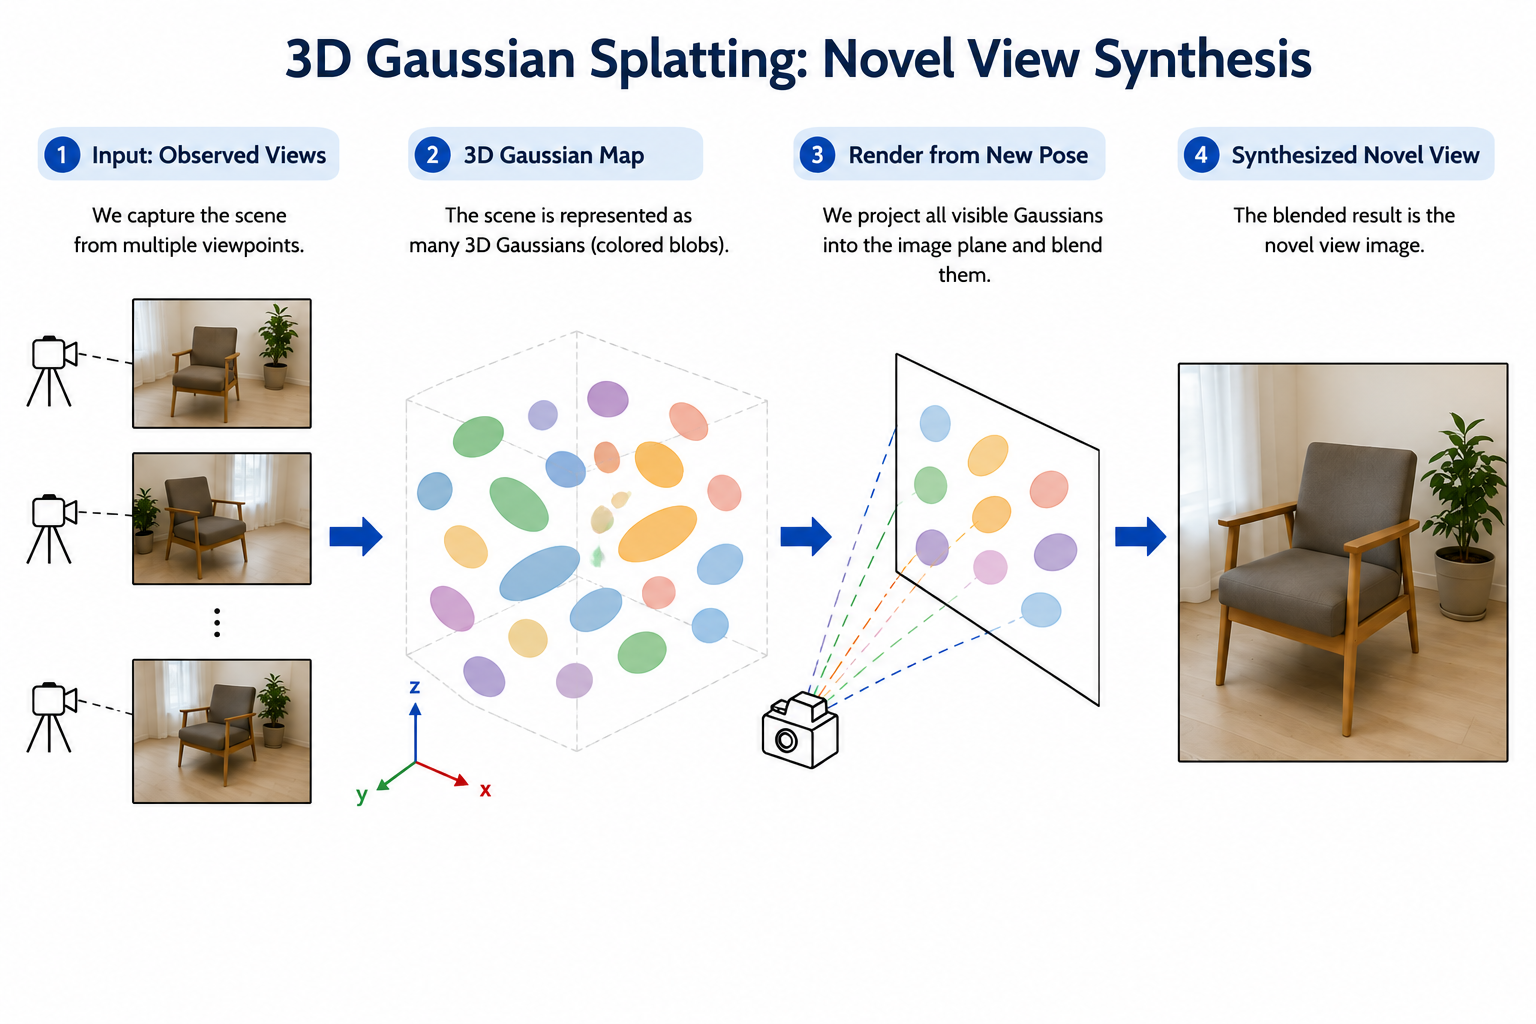
\includegraphics[width=\linewidth]{3dgs_novel_view_synthesis.png}
			\end{center}
			\end{minipage}}
		\end{column}
	\end{columns}

\end{frame}

%------------------------------------------------

\begin{frame}
	\frametitle{Why Underwater Sonar SLAM Is Hard}
	\framesubtitle{Can a renderable sonar map provide online correction factors?}

	\begin{columns}[T]
		\begin{column}{0.47\textwidth}
			\uncover<1->{\storycard{ICLBlue!6}{ICLBlue}{1. Problem setting}
			{Underwater robots cannot use GNSS. IMU/DVL odometry therefore drifts over time.}}

			\vspace{1.8mm}
			\uncover<2->{\storycard{ICLBlue!6}{ICLBlue}{2. Sensor limitation}
			{Sonar works underwater, but the image evidence is sparse, ambiguous, and viewpoint-dependent.}}

			\vspace{1.8mm}
			\uncover<3->{\storycard{ICLBlue!6}{ICLBlue}{3. Sonar-based SLAM limitation}
			{Geometric matching becomes fragile under sonar noise and repeated acoustic structure.}}
		\end{column}
		\begin{column}{0.47\textwidth}
			\uncover<4->{\storycard{ICLCream}{ICLBlue}{4. Key insight from 3DGS}
			{A learned Gaussian scene can predict the sonar view from a candidate pose.}}

			\vspace{1.8mm}
			\uncover<5->{\storycard{ICLCream}{ICLBlue}{5. Gap}
			{3DGS is rarely used as an online sonar measurement model inside SLAM.}}

			\vspace{1.8mm}
			\uncover<6->{\storycard{ICLCream}{ICLBlue}{6. Project idea}
			{Use render consistency between live sonar and 3D Gaussian Splatting prediction as a SLAM constraint.}}
		\end{column}
	\end{columns}

\end{frame}

%------------------------------------------------

\begin{frame}
	\frametitle{Research Gap: Sonar SLAM + 3DGS}

	\vspace{1mm}
	\begin{columns}[T]
		\begin{column}{0.31\textwidth}
			\uncover<1->{%
			\begin{minipage}{\linewidth}
			{\small\textbf{Underwater SLAM}}
			\begin{itemize}
				\setlength{\itemsep}{0.6mm}
				\scriptsize
				\item Fuses sonar, camera, IMU, and DVL.
				\item Uses feature, image, or sensor factors.
			\end{itemize}
			{\tiny Li et al. 2018; Cardaillac and Ludvigsen 2023; Xu et al. 2025.}
			\end{minipage}}
		\end{column}
		\begin{column}{0.31\textwidth}
			\uncover<2->{%
			\begin{minipage}{\linewidth}
			{\small\textbf{3DGS SLAM}}
			\begin{itemize}
				\setlength{\itemsep}{0.6mm}
				\scriptsize
				\item Uses Gaussian maps for tracking and reconstruction.
				\item Current systems are visual or LiDAR-based.
			\end{itemize}
			{\tiny Matsuki et al. 2024; Yan et al. 2024; Peng et al. 2024; Zhu et al. 2025.}
			\end{minipage}}
		\end{column}
		\begin{column}{0.31\textwidth}
			\uncover<3->{%
			\begin{minipage}{\linewidth}
			{\small\textbf{Underwater 3DGS}}
			\begin{itemize}
				\setlength{\itemsep}{0.6mm}
				\scriptsize
				\item Models underwater camera or sonar appearance.
				\item Focuses on reconstruction and rendering, not SLAM.
			\end{itemize}
			{\tiny Ling et al. 2025; Yang et al. 2025; Li et al. 2025; Xu et al. 2026.}
			\end{minipage}}
		\end{column}
	\end{columns}

	\vspace{5mm}
	\onslide<4->
	\begin{center}
		\setlength{\fboxsep}{5pt}
		\fcolorbox{ICLBlue}{ICLCream}{%
			\begin{minipage}{0.90\textwidth}
				\centering
				{\small\textbf{Missing integration in the reviewed literature}}\par\vspace{0.8mm}
				{\footnotesize Live sonar \(\rightarrow\) sonar 3DGS candidate render \(\rightarrow\) gated Pose3 factor \(\rightarrow\) iSAM2.}
			\end{minipage}}
	\end{center}
\end{frame}

%------------------------------------------------

\begin{frame}
	\frametitle{NAS-GS: Noise-Aware Sonar Gaussian Splatting}
	\framesubtitle{A renderable sonar measurement model reference}

	\begin{columns}[T]
		\begin{column}{0.58\textwidth}
			\vspace{-1mm}
			\begin{center}
				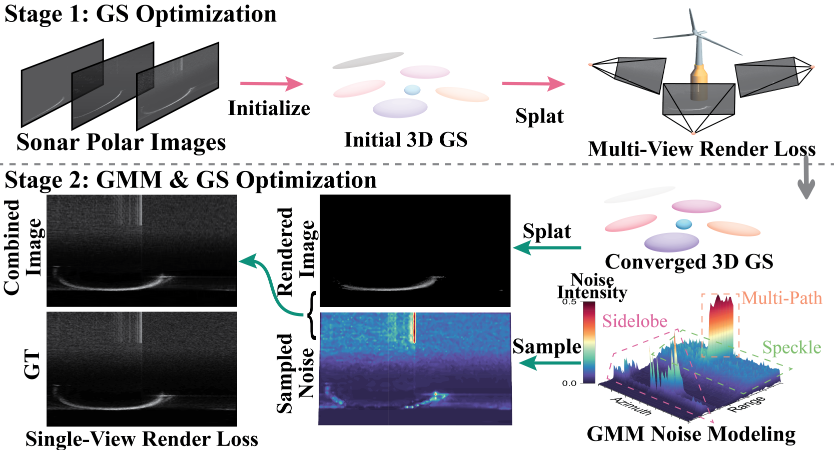
\includegraphics[width=\linewidth]{nasgs_pipeline_overview.png}

				\vspace{0.5mm}
				{\scriptsize NAS-GS training pipeline, adapted from Xu et al.}
			\end{center}
		\end{column}
		\begin{column}{0.38\textwidth}
			{\large\textbf{What NAS-GS does}}

			\vspace{1mm}
			\begin{itemize}
				\setlength{\itemsep}{1.4mm}
				\footnotesize
				\item Learns a 3D Gaussian sonar scene from polar sonar images.
				\item Optimises rendered structure together with acoustic noise appearance.
				\item Produces a differentiable sonar renderer for new viewpoints.
			\end{itemize}

			\vspace{2mm}
			{\large\textbf{How I use it}}

			\vspace{1mm}
			\begin{itemize}
				\setlength{\itemsep}{1.4mm}
				\footnotesize
				\item Freeze the trained map during replay.
				\item Render candidate Pose3 hypotheses online.
				\item Insert a factor only when live sonar and render agree.
			\end{itemize}
		\end{column}
	\end{columns}

\end{frame}

%------------------------------------------------

\begin{frame}
	\frametitle{SLAM Pose graph optimization with Pose3 constraints and iSAM2 backend}
	\framesubtitle{NAS-GS predicts observations; iSAM2 consumes accepted constraints}

	\begin{center}
		\small
		\textbf{Online loop:}
		render from the map, compare with the live frame, then add a graph factor only when the evidence is strong.
	\end{center}

	\vspace{1.5mm}

	\begin{columns}[T]
		\begin{column}{0.31\textwidth}
			\onslide<1->
			\storycard{ICLBlue!6}{ICLBlue}{Renderable sonar map}
			{NAS-GS predicts what the sonar should observe from a proposed Pose3 camera pose.}

			\vspace{2mm}
			\begin{center}
				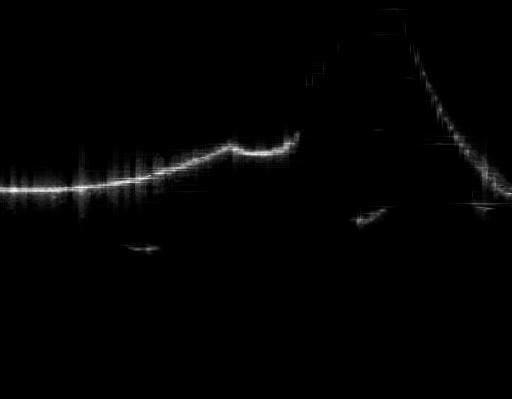
\includegraphics[width=0.92\linewidth,height=0.28\textheight,keepaspectratio]{slide_posegraph_sonar_map.png}
			\end{center}
		\end{column}
		\begin{column}{0.31\textwidth}
			\onslide<2->
			\storycard{ICLBlue!6}{ICLBlue}{Online evidence}
			{A live sonar frame is compared against rendered candidates around the current drifted pose.}

			\vspace{2mm}
			\begin{center}
				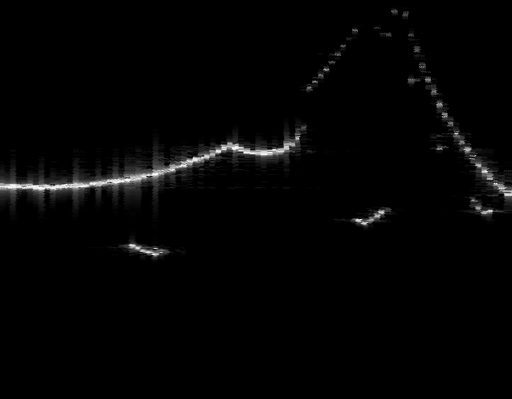
\includegraphics[width=0.92\linewidth,height=0.28\textheight,keepaspectratio]{slide_posegraph_live_sonar.png}
			\end{center}
		\end{column}
		\begin{column}{0.31\textwidth}
			\onslide<3->
			\storycard{ICLBlue!6}{ICLBlue}{Graph correction}
			{If render similarity and gates pass, the recovered pose is inserted as a Pose3 factor.}

			\vspace{2mm}
			\begin{center}
				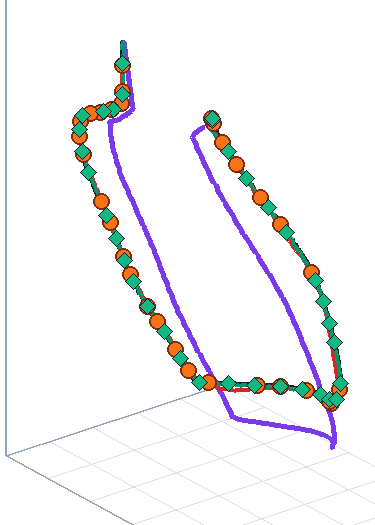
\includegraphics[width=0.92\linewidth,height=0.28\textheight,keepaspectratio]{slide_render_consistency_corrected_graph.png}
			\end{center}
		\end{column}
	\end{columns}
\end{frame}

%------------------------------------------------

\begin{frame}
	\frametitle{Online-render Registration Backbone}
	\framesubtitle{Same online loop for same-route correction and revisit correction}

	\vspace{1mm}
	\begin{center}
		\begin{tikzpicture}[
			box/.style={draw=ICLBlue, fill=ICLBlue!7, rounded corners=2pt, align=center, minimum height=1.05cm, text width=2.05cm, font=\scriptsize},
			arrow/.style={->, line width=0.9pt, draw=ICLBlue},
			node distance=0.42cm
		]
			\node[box] (live) at (0,0) {Live replay\\sonar + Pose3};
			\node[box] (cand) at (2.35,0) {Candidate\\poses};
			\node[box] (render) at (4.70,0) {NAS-GS\\render};
			\node[box] (score) at (7.05,0) {Score\\and gate};
			\node[box] (factor) at (9.40,0) {Pose3\\factor};
			\node[box] (graph) at (11.75,0) {iSAM2\\update};
			\draw[arrow] (live) -- (cand);
			\draw[arrow] (cand) -- (render);
			\draw[arrow] (render) -- (score);
			\draw[arrow] (score) -- (factor);
			\draw[arrow] (factor) -- (graph);
		\end{tikzpicture}
	\end{center}

	\vspace{3mm}
	\begin{columns}[T]
		\begin{column}{0.44\textwidth}
			\storycard{ICLBlue!6}{ICLBlue}{Local single}
			{Compact \(x,y,z,\psi\) search around the live Pose3 baseline for nearby pose correction.}
		\end{column}
		\begin{column}{0.44\textwidth}
			\storycard{ICLCream}{ICLBlue}{Route-progress revisit}
			{Ordered sequence render search guided by route progress and drift-prior checks.}
		\end{column}
	\end{columns}

	\vspace{3mm}
	{\footnotesize
	Gating is configured separately from the search mode. Score and structure checks prevent weak render matches from entering the graph.
	}
\end{frame}

%------------------------------------------------

\begin{frame}
	\frametitle{Algorithm Step 1: Live Replay System}

	\vspace{-1mm}
	\begin{center}
		\begin{tikzpicture}[
			pub/.style={draw=ICLBlue, fill=ICLBlue!7, rounded corners=2pt, align=center, minimum height=0.78cm, text width=1.75cm, font=\scriptsize},
			bus/.style={draw=ICLBlue, fill=white, rounded corners=2pt, align=left, minimum height=1.35cm, text width=1.75cm, font=\tiny},
			node/.style={draw=ICLBlue, fill=ICLCream, rounded corners=2pt, align=center, minimum height=0.72cm, text width=2.0cm, font=\scriptsize},
			output/.style={draw=orange, fill=orange!12, rounded corners=2pt, align=center, minimum height=0.54cm, text width=1.68cm, font=\tiny},
			arrow/.style={->, line width=0.75pt, draw=ICLBlue},
			query/.style={->, line width=1.0pt, draw=orange, dashed}
		]

			% ROS replay
			\node[pub] (bag) at (0,1.35) {rosbag\\replay};
			\node[bus] (bus) at (2.55,1.35) {\textbf{ROS topics}\\[-0.2mm]
				/sonar/image\\
				/imu, /dvl\\
				/tf, /GT};

			% SLAM pipeline nodes
			\node[node] (odom) at (5.30,2.35) {IMU/DVL\\odometry};
			\node[node] (reg) at (5.30,1.10) {online-render\\registration};
			\node[node] (render) at (5.30,-0.15) {GS\_Sonar\\render service};

			% SLAM backend (space increased)
			\node[node] (isam) at (10.15,1.75) {Pose3 backend\\iSAM2};
			\node[output] (corrected) at (13.10,1.75) {corrected\\Pose3};

			% outputs
			\node[output] (baseline) at (7.85,2.35) {baseline\\Pose3};
			\node[output] (factor) at (7.85,1.10) {registration\\factor};
			\node[node] (eval) at (10.15,0.35) {evaluation\\subscriber};

			% labels
			\node[font=\tiny, color=ICLDarkBlue] at (2.55,2.82) {published by replay};
			\node[font=\tiny, color=ICLDarkBlue] at (5.30,2.82) {subscribers};
			\node[font=\tiny, color=ICLDarkBlue] at (8.95,2.82) {factor graph};

			% ROS flow
			\draw[arrow] (bag) -- (bus);
			\draw[arrow] (bus.east) -- ++(0.35,0) |- (odom.west);
			\draw[arrow] (bus.east) -- ++(0.35,0) |- (reg.west);
			\draw[arrow] (bus.east) -- ++(0.35,0) |- (eval.west);

			% odometry to SLAM
			\draw[arrow] (odom) -- (baseline);
			\draw[arrow] (baseline) -- (isam);

			% registration pipeline
			\draw[query] (reg) -- (render);
			\draw[arrow] (reg) -- (factor);

			% factor graph to backend
			\draw[arrow] (factor.east) -- (isam.west);

			% SLAM output
			\draw[arrow] (isam) -- (corrected);

			% evaluation
			\draw[arrow] (corrected.south) -- (eval.north);

		\end{tikzpicture}
	\end{center}

	\vspace{1mm}
	{\footnotesize
	The replay is deliberately online. Nodes subscribe to ROS topics in time order, the registration node queries NAS-GS only at candidate poses, and iSAM2 receives only gated Pose3 factors.
	}
\end{frame}
%------------------------------------------------

\begin{frame}
	\frametitle{Algorithm Step 2: Candidate Pose And NAS-GS Render}

	\begin{columns}[T]
		\begin{column}{0.32\textwidth}
			{\small\textbf{Local single-frame search}}
			\vspace{1mm}
			\begin{center}
				\begin{tikzpicture}[scale=0.66]
					\draw[step=0.55, color=ICLBlue!18] (-1.7,-1.7) grid (1.7,1.7);
					\draw[line width=1.2pt, color=ICLBlue] (-1.45,-1.0) .. controls (-0.5,-0.5) and (0.35,0.45) .. (1.35,0.9);
					\foreach \x in {-0.8,0,0.8} {
						\foreach \y in {-0.8,0,0.8} {
							\fill[orange] (\x,\y) circle (2.2pt);
						}
					}
					\fill[ICLDarkBlue] (0,0) circle (3.0pt);
					\node[font=\tiny, align=center] at (0,-2.05) {single live frame\\around baseline};
				\end{tikzpicture}
			\end{center}
			{\scriptsize Compact \(x,y,z,\psi\) grid for same-route correction.}
		\end{column}
		\begin{column}{0.32\textwidth}
			{\small\textbf{Route-progress sequence search}}
			\vspace{1mm}
			\begin{center}
				\begin{tikzpicture}[scale=0.66]
					\draw[step=0.55, color=ICLBlue!18] (-1.7,-1.7) grid (1.7,1.7);
					\draw[line width=1.2pt, color=ICLBlue] (-1.45,-1.1) .. controls (-0.5,0.05) and (0.35,0.65) .. (1.45,1.05);
					\draw[line width=1.0pt, color=orange] (-1.35,-0.75) .. controls (-0.25,0.25) and (0.55,0.35) .. (1.35,0.75);
					\foreach \x in {-1.1,-0.55,0,0.55,1.1} {
						\foreach \y in {-1.1,-0.55,0,0.55,1.1} {
							\fill[orange!80] (\x,\y) circle (1.6pt);
						}
					}
					\draw[rounded corners=1pt, draw=ICLBlue, fill=white] (-1.45,1.55) rectangle (-0.85,1.9);
					\draw[rounded corners=1pt, draw=ICLBlue, fill=white] (-0.25,1.55) rectangle (0.35,1.9);
					\draw[rounded corners=1pt, draw=ICLBlue, fill=white] (0.95,1.55) rectangle (1.55,1.9);
					\node[font=\tiny] at (-1.15,2.08) {$t-1$};
					\node[font=\tiny] at (0.05,2.08) {$t$};
					\node[font=\tiny] at (1.25,2.08) {$t+1$};
					\node[font=\tiny, align=center] at (0,-2.05) {sequence evidence\\around route prior};
				\end{tikzpicture}
			\end{center}
			{\scriptsize The orange line is a smooth candidate correction sequence. Wider candidates are allowed, but neighbouring frames must agree.}
		\end{column}
		\begin{column}{0.31\textwidth}
			{\small\textbf{Render query}}
			\vspace{1mm}
			\begin{center}
				\begin{tikzpicture}
					\node[draw=ICLBlue, fill=ICLCream, rounded corners=2pt, align=center, text width=2.5cm, minimum height=0.85cm, font=\scriptsize] (server) at (0,0.7) {GS\_Sonar\\render server};
					\node[draw=ICLBlue, fill=ICLBlue!7, rounded corners=2pt, align=center, text width=2.5cm, minimum height=0.7cm, font=\scriptsize] (pose) at (0,2.0) {picked Pose3\\candidate};
					\draw[->, line width=0.8pt, draw=ICLBlue] (pose) -- (server);
				\end{tikzpicture}
				\vspace{1mm}
				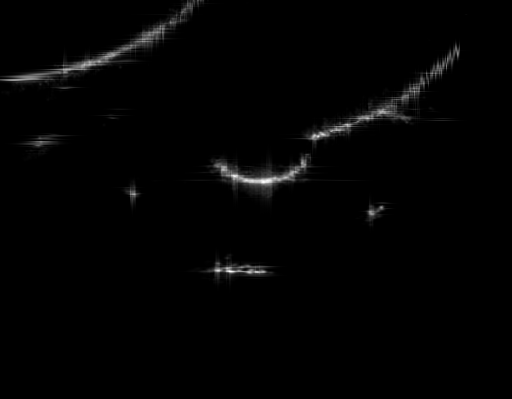
\includegraphics[width=0.95\linewidth,height=0.23\textheight,keepaspectratio]{slide_step2_random_rendered_sonar.png}
			\end{center}
			{\scriptsize The output is a rendered sonar image for the proposed robot pose.}
		\end{column}
	\end{columns}
\end{frame}

%------------------------------------------------

\begin{frame}
	\frametitle{Algorithm Step 3: Score And Gate}

	\begin{columns}[T]
		\begin{column}{0.47\textwidth}
			{\small\textbf{Accepted pair}}
			\vspace{1mm}
			\begin{columns}[T,totalwidth=\linewidth]
				\begin{column}{0.49\linewidth}
					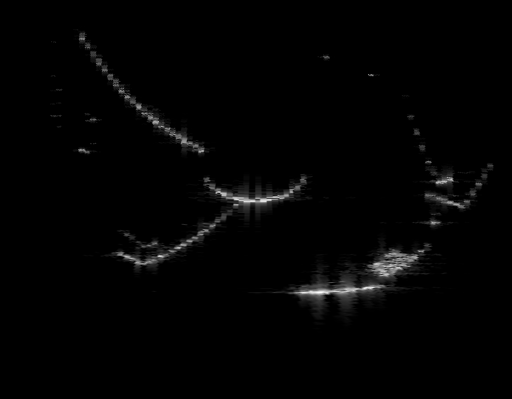
\includegraphics[width=\linewidth,height=0.205\textheight,keepaspectratio]{slide_render_consistency_live_sonar.png}
					\par\vspace{0.5mm}{\centering\tiny live sonar\par}
				\end{column}
				\begin{column}{0.49\linewidth}
					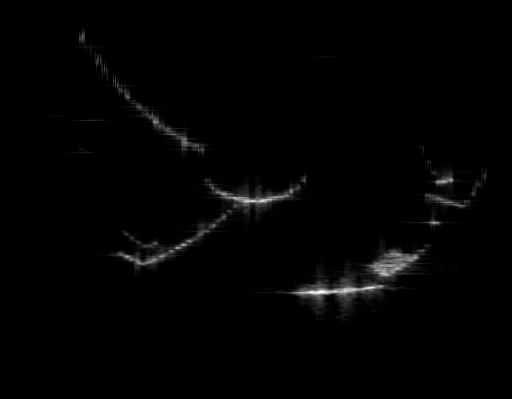
\includegraphics[width=\linewidth,height=0.205\textheight,keepaspectratio]{slide_render_consistency_sonar_map.png}
					\par\vspace{0.5mm}{\centering\tiny rendered sonar\par}
				\end{column}
			\end{columns}
			\vspace{1mm}
			{\scriptsize Frame 24 selects rendered frame 24 and passes the score gate.}
			\vspace{0.5mm}

			{\tiny
			\begin{tabular}{@{}ll@{}}
				score gate & \(s=0.926 \geq 0.08\), pass\\
				pose gate & shift \(=0.048\) m, pass\\
				replay evidence & published as a Pose3 registration factor
			\end{tabular}}
		\end{column}
		\begin{column}{0.47\textwidth}
			{\small\textbf{Rejected pair}}
			\vspace{1mm}
			\begin{columns}[T,totalwidth=\linewidth]
				\begin{column}{0.49\linewidth}
					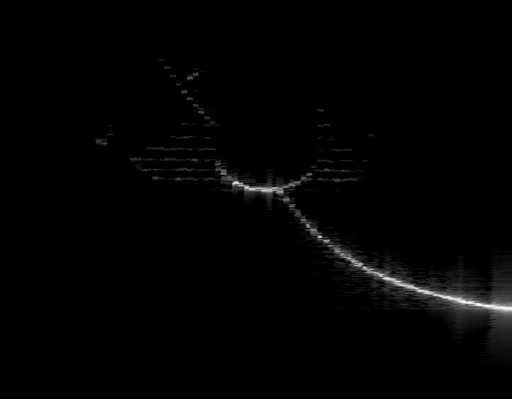
\includegraphics[width=\linewidth,height=0.205\textheight,keepaspectratio]{slide_score_reject_live.png}
					\par\vspace{0.5mm}{\centering\tiny live sonar\par}
				\end{column}
				\begin{column}{0.49\linewidth}
					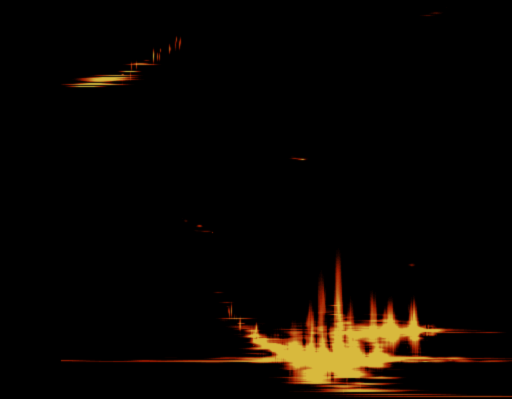
\includegraphics[width=\linewidth,height=0.205\textheight,keepaspectratio]{slide_score_reject_render.png}
					\par\vspace{0.5mm}{\centering\tiny rendered sonar\par}
				\end{column}
			\end{columns}
			\vspace{1mm}
			{\scriptsize Frame 228 selects rendered frame 216 but falls just below threshold.}
			\vspace{0.5mm}

			{\tiny
			\begin{tabular}{@{}ll@{}}
				score gate & \(s=0.0799 < 0.08\), fail\\
				edge check & best candidate on search edge\\
				replay evidence & one of 6 score-below-threshold events
			\end{tabular}}
		\end{column}
	\end{columns}

	\vspace{1mm}
	\begin{columns}[T]
		\begin{column}{0.47\textwidth}
			{\scriptsize\textbf{Score calculation}}\\[-0.5mm]
			{\tiny Intensity normalisation, NCC-style similarity, residual penalty, and bright-return overlap are combined into one render score. Minimum threshold \(s_{\min}=0.08\).}
		\end{column}
		\begin{column}{0.47\textwidth}
			{\scriptsize\textbf{Gates before insertion}}\\[-0.5mm]
			{\tiny Render-score, structure-support, pose-jump, and temporal-consistency gates must pass before publishing a Pose3 factor to iSAM2.}
		\end{column}
	\end{columns}
\end{frame}

%------------------------------------------------

\begin{frame}
	\frametitle{Algorithm Step 4: Pose3 Factor And iSAM2 Update}

	\begin{columns}[T]
		\begin{column}{0.58\textwidth}
			\begin{center}
				\begin{tikzpicture}[scale=0.84]
					\foreach \i/\x/\y in {0/0/0,1/1.3/0.15,2/2.6/0.0,3/3.9/0.35,4/5.2/0.25} {
						\filldraw[fill=ICLBlue!12, draw=ICLBlue, line width=0.9pt] (\x,\y) circle (0.13);
						\node[font=\tiny] at (\x,\y-0.35) {$X_{\i}$};
					}
					\draw[->, line width=1.0pt, draw=ICLBlue] (0.13,0.02) -- (1.17,0.14);
					\draw[->, line width=1.0pt, draw=ICLBlue] (1.43,0.14) -- (2.47,0.02);
					\draw[->, line width=1.0pt, draw=ICLBlue] (2.73,0.03) -- (3.77,0.31);
					\draw[->, line width=1.0pt, draw=ICLBlue] (4.03,0.34) -- (5.07,0.27);
					\node[draw=orange, fill=orange!15, rounded corners=2pt, align=center, text width=2.2cm, font=\scriptsize] (nasgs) at (3.9,1.85) {accepted\\NAS-GS pose};
					\draw[->, line width=1.1pt, draw=orange] (nasgs) -- node[right, font=\tiny] {Pose3 factor} (3.9,0.52);
					\draw[line width=1.1pt, draw=ICLBlue!45, dashed] (0,-0.85) .. controls (1.3,-1.0) and (2.6,-0.95) .. (3.9,-0.78) .. controls (4.7,-0.68) .. (5.3,-0.55);
					\node[font=\tiny, color=ICLBlue] at (1.35,-1.28) {before factor};
					\draw[line width=1.3pt, draw=red] (0,-0.55) .. controls (1.4,-0.45) and (2.5,-0.37) .. (3.9,-0.10) .. controls (4.5,0.02) .. (5.2,0.12);
					\node[font=\tiny, color=red] at (5.0,-0.30) {after iSAM2 update};
				\end{tikzpicture}
			\end{center}
		\end{column}
		\begin{column}{0.36\textwidth}
			\storycard{ICLBlue!6}{ICLBlue}{Before}
			{The graph contains IMU/DVL odometry factors, so drift accumulates along the chain.}

			\vspace{2mm}
			\storycard{ICLCream}{ICLBlue}{Insertion}
			{The accepted candidate pose and covariance are published as a Pose3 registration factor.}

			\vspace{2mm}
			\storycard{ICLBlue!6}{ICLBlue}{After}
			{iSAM2 optimises the graph, pulling nearby states toward the render-consistent pose.}
		\end{column}
	\end{columns}
\end{frame}

%------------------------------------------------

\begin{frame}
	\frametitle{Algorithm Step 5: Route-progress Revisit Priors}

	\vspace{-1mm}
	\begin{center}
		\begin{tikzpicture}[
			box/.style={draw=ICLBlue, fill=ICLBlue!7, rounded corners=2pt, align=center, minimum height=0.55cm, text width=1.80cm, font=\tiny},
			prior/.style={draw=orange, fill=orange!12, rounded corners=2pt, align=center, minimum height=0.55cm, text width=1.85cm, font=\tiny},
			arrow/.style={->, line width=0.8pt, draw=ICLBlue}
		]
			\node[box] (seq) at (0,0) {Pass B\\window};
			\node[prior] (route) at (2.15,0) {route progress\\selects map window};
			\node[prior] (drift) at (4.55,0) {drift prior\\checks envelope};
			\node[box] (search) at (6.95,0) {sequence\\render search};
			\node[box] (gate) at (9.10,0) {score\\and gate};
			\node[box] (factor) at (11.25,0) {Pose3\\factor};
			\draw[arrow] (seq) -- (route);
			\draw[arrow] (route) -- (drift);
			\draw[arrow] (drift) -- (search);
			\draw[arrow] (search) -- (gate);
			\draw[arrow] (gate) -- (factor);
		\end{tikzpicture}
	\end{center}

	\vspace{0.5mm}
	\begin{columns}[T]
		\begin{column}{0.43\textwidth}
			{\small\textbf{Route prior}}
			{\scriptsize
			\begin{itemize}
				\setlength{\itemsep}{1.2mm}
				\item Express the current revisit frame as normalised route progress from 0 to 1.
				\item Select the corresponding ordered window on the mapping route instead of trusting the nearest drifted pose.
				\item Use this window only as a proposal; sequence render evidence selects the final factor pose.
			\end{itemize}
			}
		\end{column}
		\begin{column}{0.53\textwidth}
			{\small\textbf{Drift prior}}
			{\scriptsize
			\begin{itemize}
				\setlength{\itemsep}{1.0mm}
				\item Learn expected drift magnitude from aligned baseline-to-GT errors, using 21-sample smoothing and a PCHIP curve over travelled distance.
				\item Query absolute XY, z, and yaw magnitudes at the current distance, allowing transfer when route direction changes.
				\item Reject only excess beyond the learned envelope: 3.0 m XY, 2.5 m z, or 0.70 rad yaw. NAS-GS selects the pose inside it.
			\end{itemize}
			}
		\end{column}
	\end{columns}
\end{frame}

%------------------------------------------------


%------------------------------------------------

\begin{frame}
	\frametitle{Simulation Platform: DAVE In Docker}
	\framesubtitle{Repeatable sonar, IMU, DVL, and ground-truth recording}

	\begin{columns}[T]
		\begin{column}{0.44\textwidth}
			{\normalsize\textbf{Docker setting and robot model}}
			\vspace{0.8mm}
			\begin{itemize}
				\setlength{\itemsep}{1.0mm}
				\scriptsize
				\item CUDA-enabled Docker container.
				\item DAVE with ROS Noetic and Gazebo.
				\item BlueROV2 vehicle model.
				\item Sensors recorded: sonar, IMU, DVL, odometry, and pose ground truth.
			\end{itemize}

			\vspace{3mm}
			{\normalsize\textbf{Custom scene description}}
			\vspace{0.8mm}
			\begin{itemize}
				\setlength{\itemsep}{1.0mm}
				\scriptsize
				\item A fixed underwater target structure creates repeatable sonar returns.
				\item Pass A, Pass A revisit, and Pass B use controlled waypoint routes.
				\item Sonar field of view, range, beam pattern, and noise are explicitly set.
			\end{itemize}
		\end{column}
		\begin{column}{0.52\textwidth}
			\begin{center}
				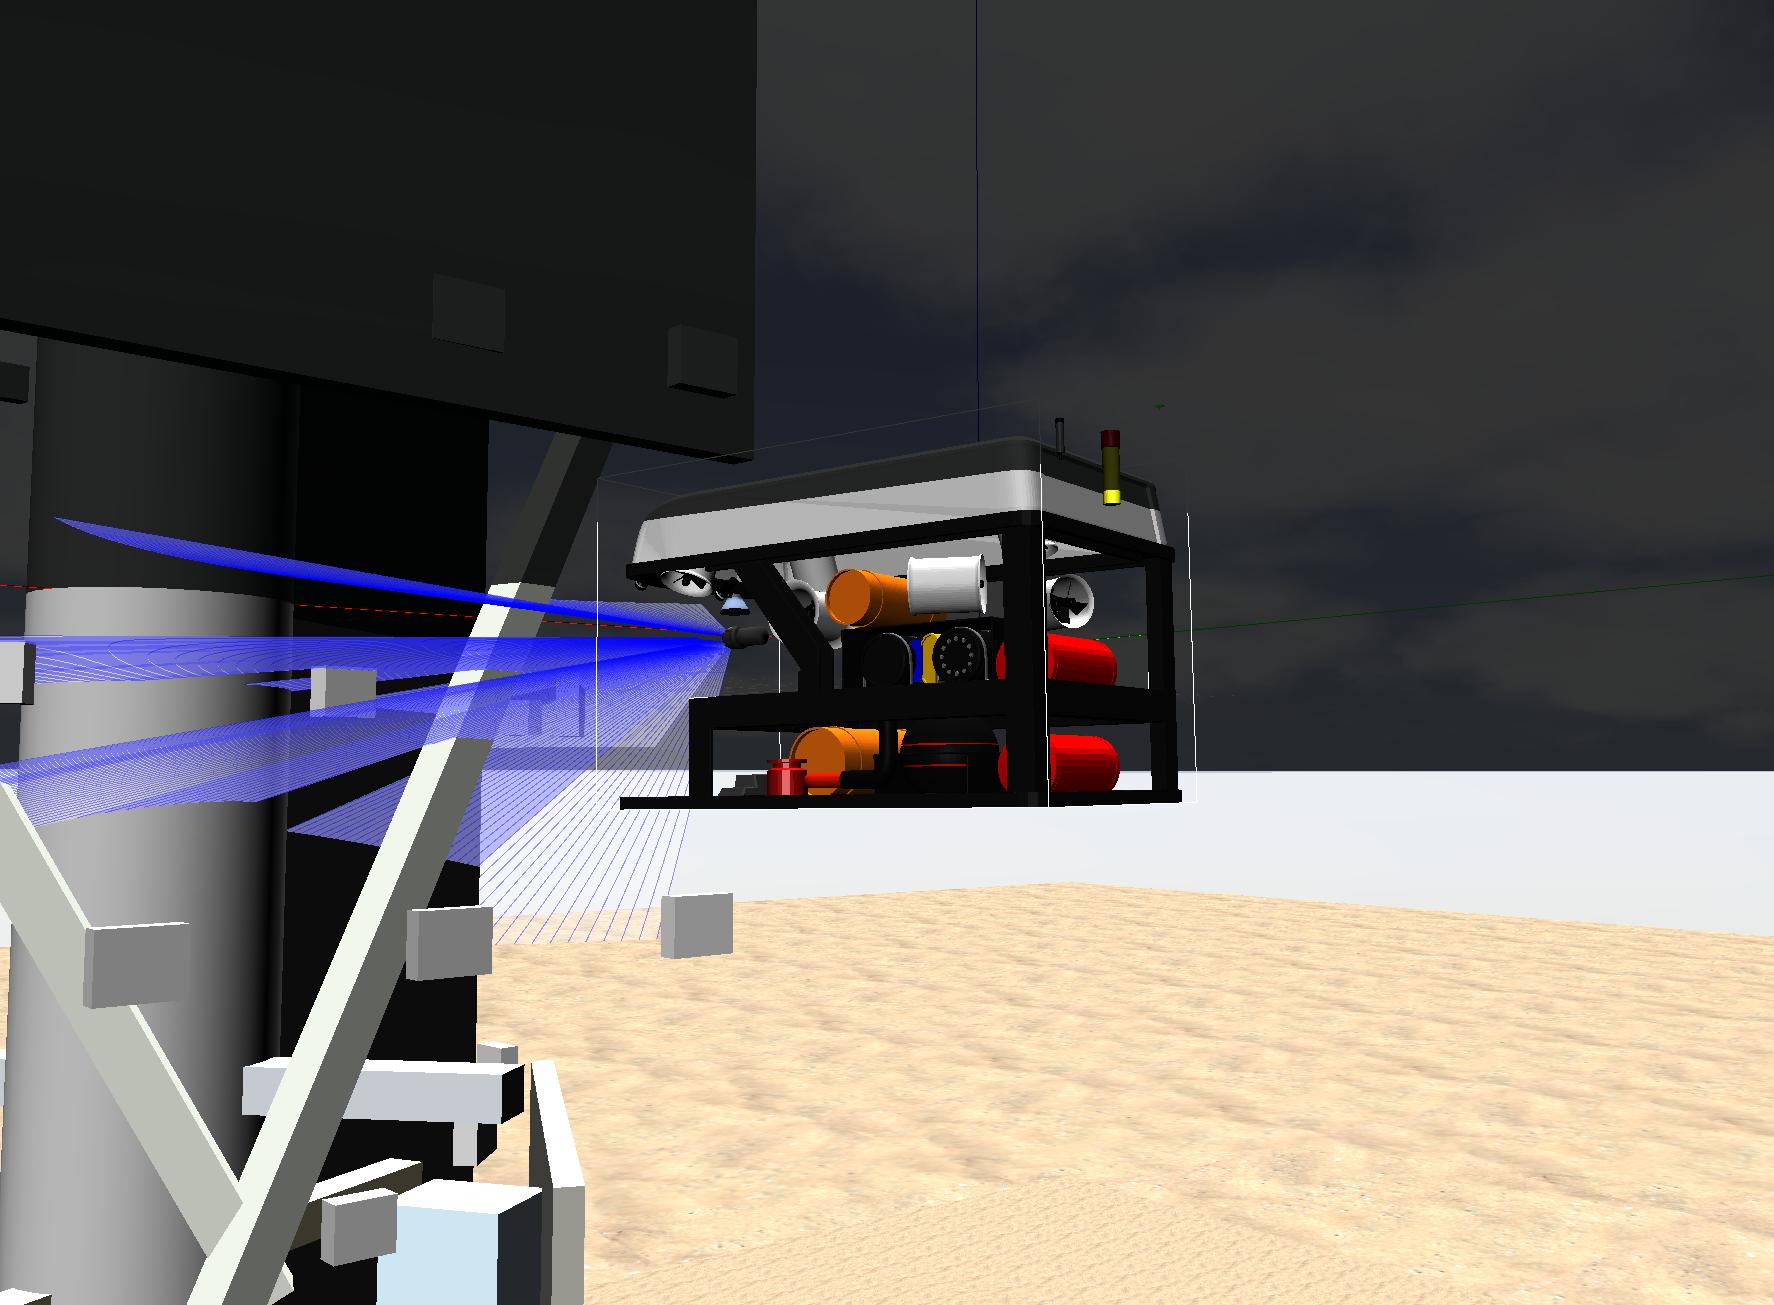
\includegraphics[width=0.70\linewidth,height=0.3\textheight,keepaspectratio]{dave_gazebo_scene_overview.jpg}
				\hfill
				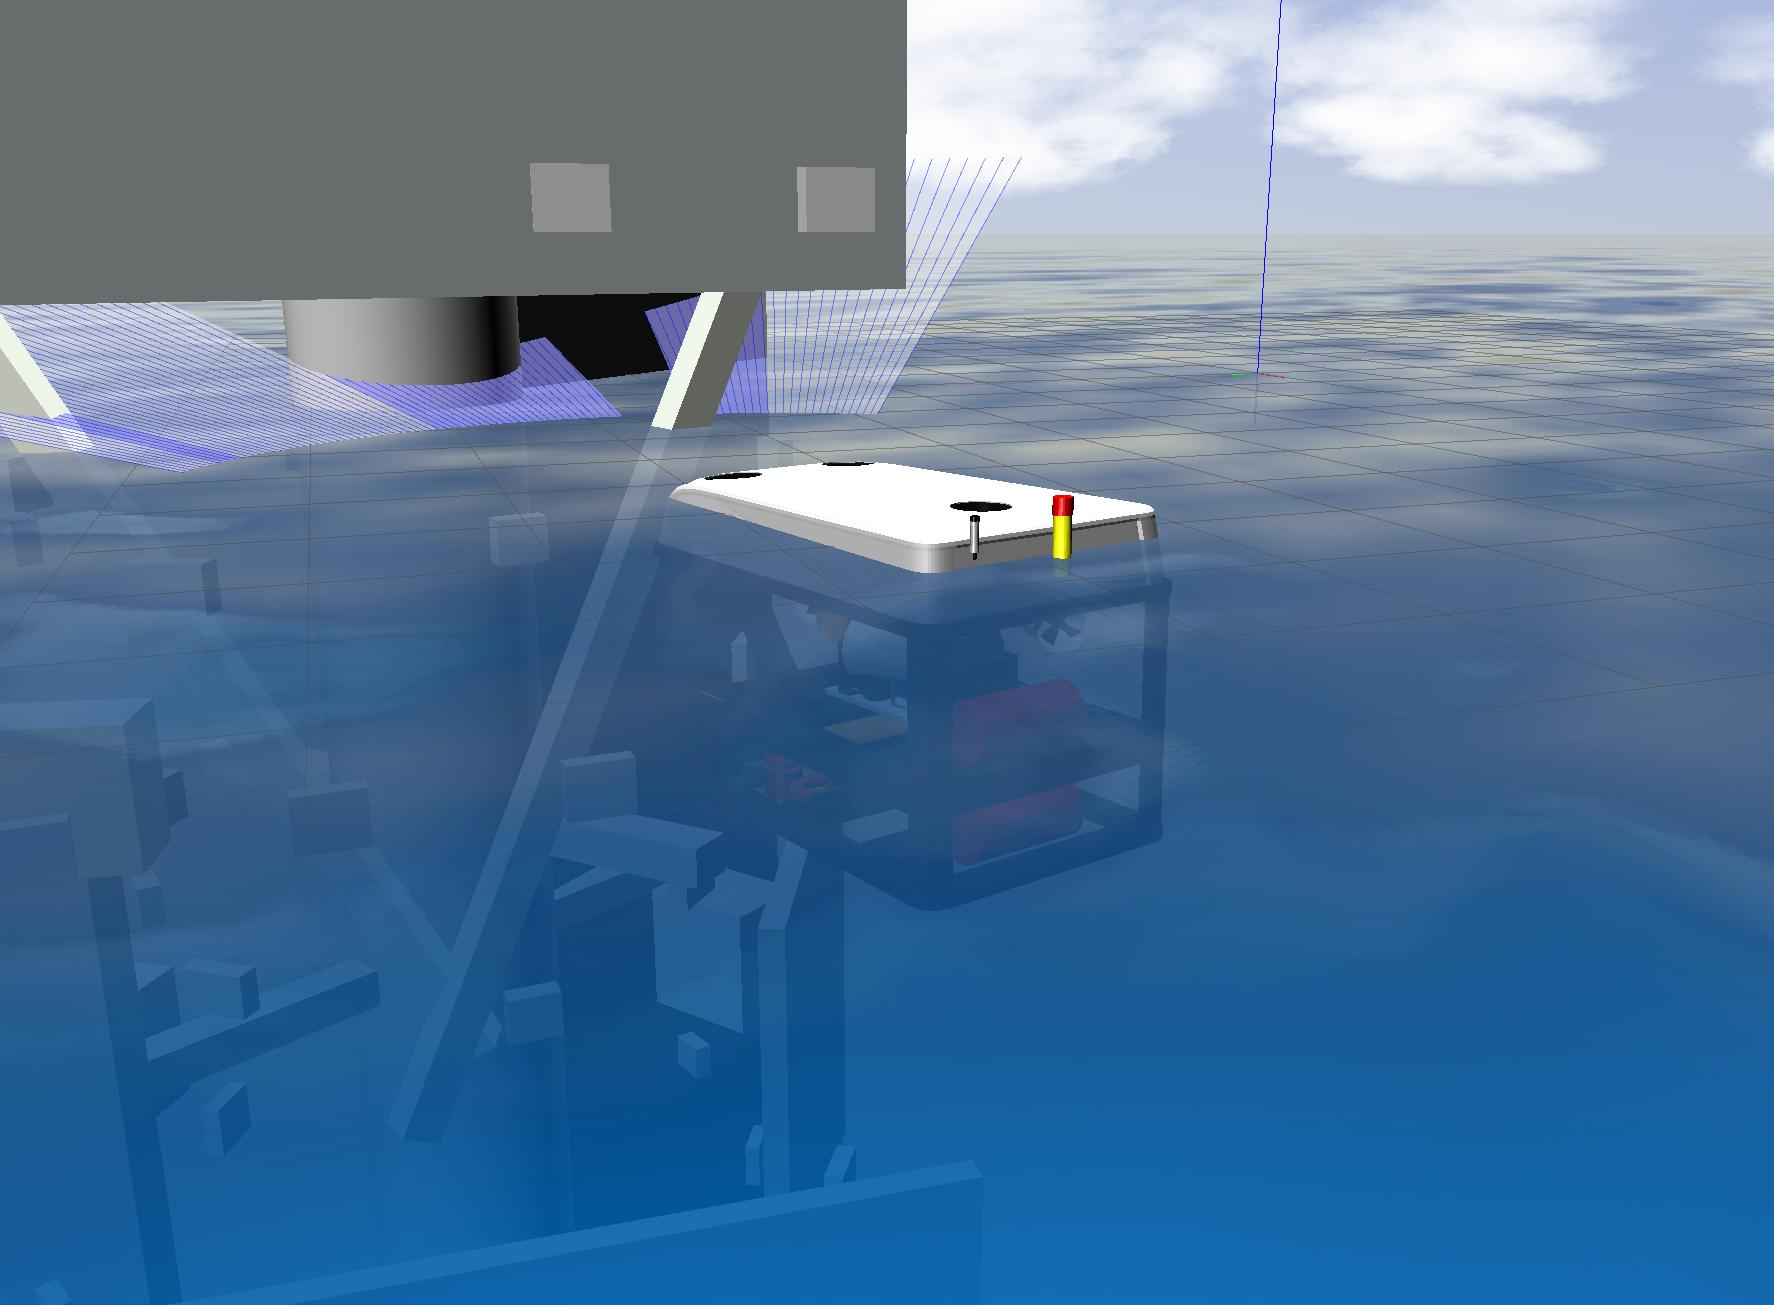
\includegraphics[width=0.70\linewidth,height=0.3\textheight,keepaspectratio]{dave_gazebo_target_scene.jpg}

				\vspace{3mm}
				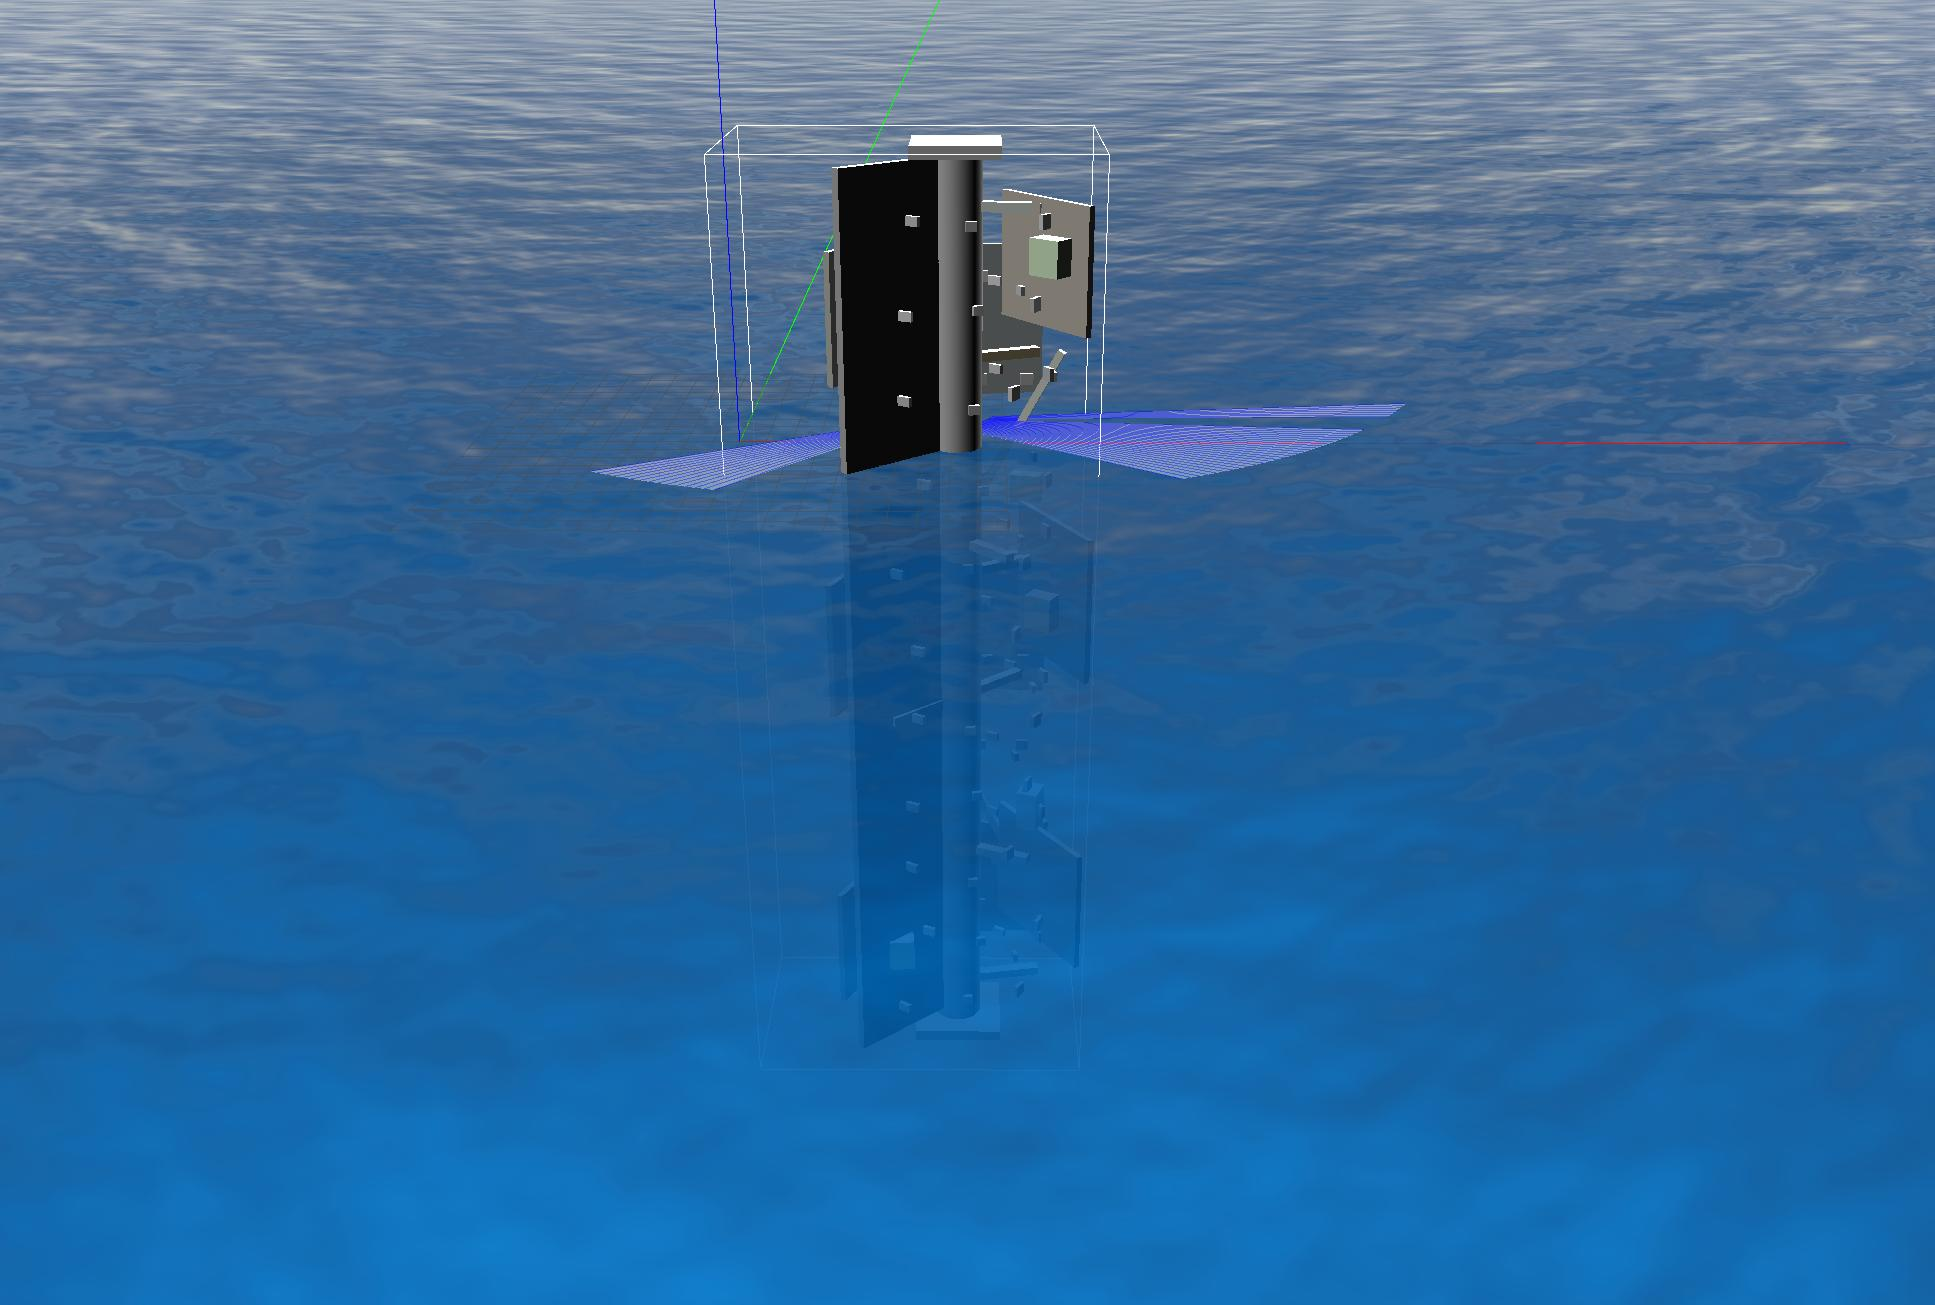
\includegraphics[width=0.70\linewidth,height=0.3\textheight,keepaspectratio]{dave_gazebo_recording_vehicle.jpg}
			\end{center}
		\end{column}
	\end{columns}
\end{frame}

%------------------------------------------------

\begin{frame}
	\frametitle{Simulation Path Recording}
	\framesubtitle{Pass A trains the map; Pass B reuses the start point but follows a hard revisit path}

	\vspace{-1mm}
	\begin{columns}[T]
		\begin{column}{0.64\textwidth}
			\begin{center}
				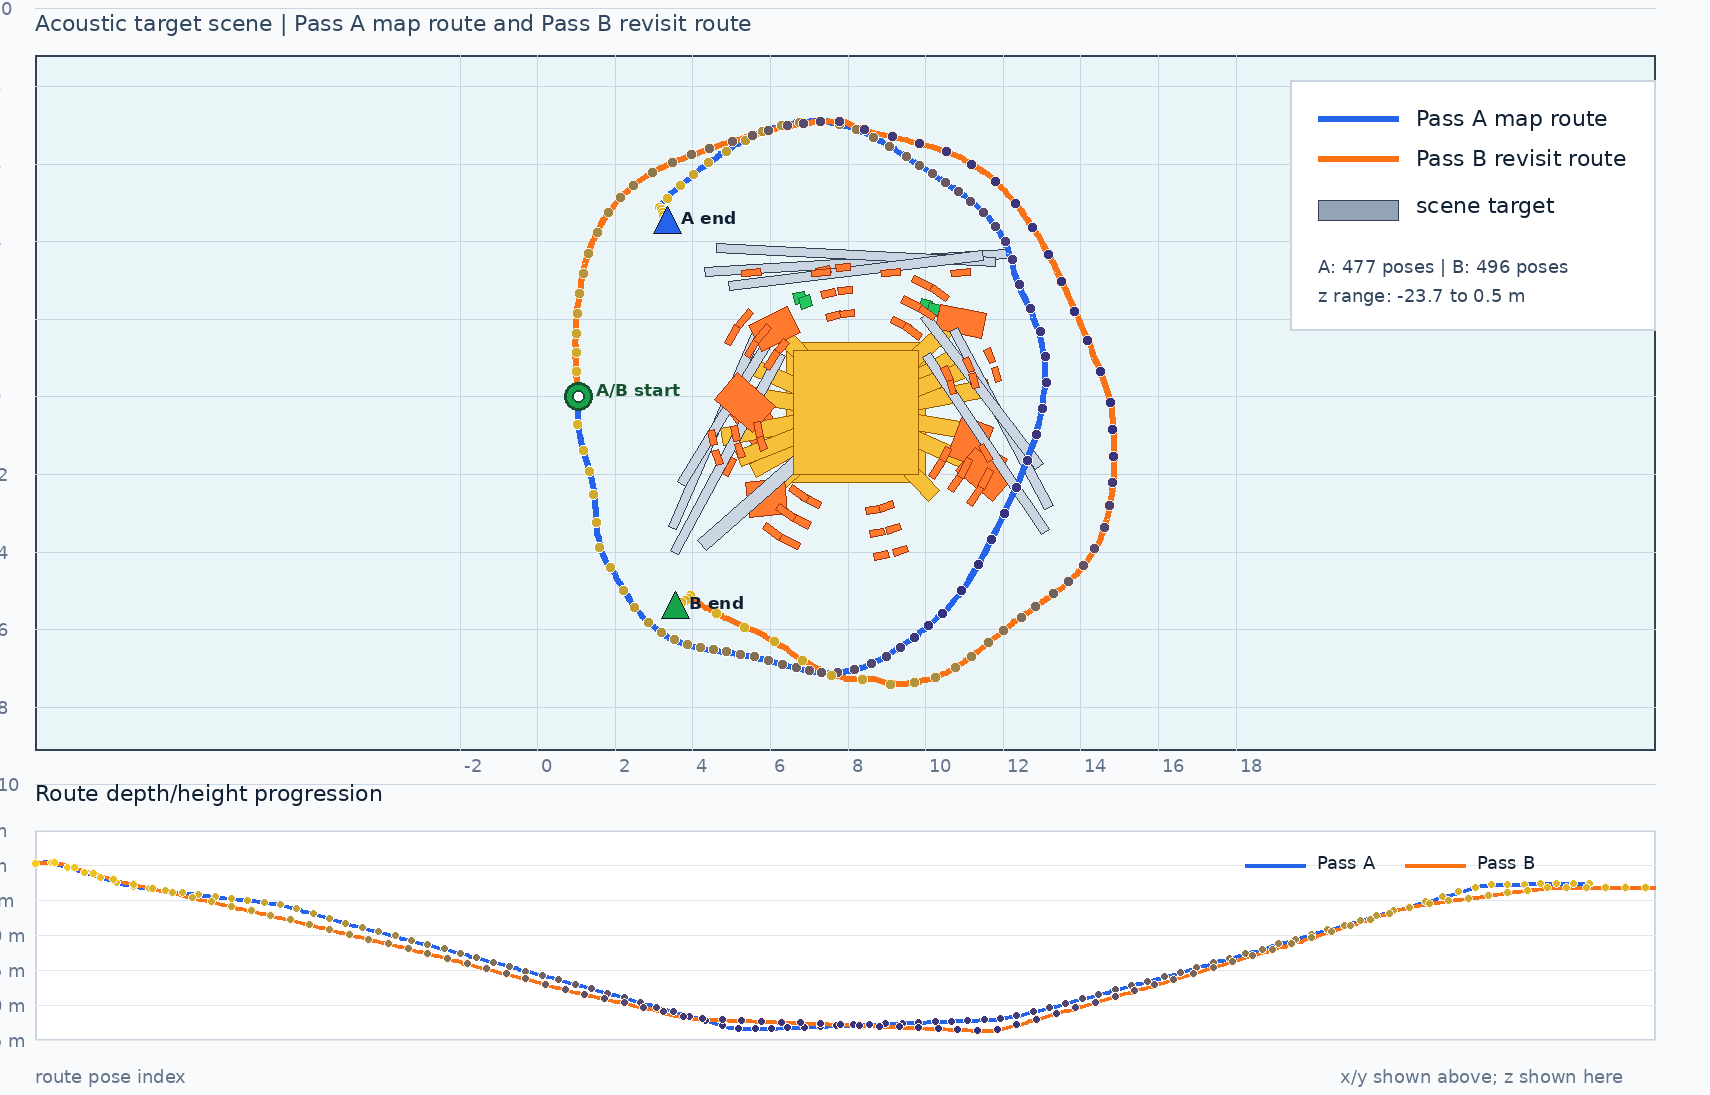
\includegraphics[width=\linewidth,height=0.73\textheight,keepaspectratio]{passA_passB_route_top_view_slidecrop.png}
			\end{center}
		\end{column}
		\begin{column}{0.32\textwidth}
			\begin{center}
				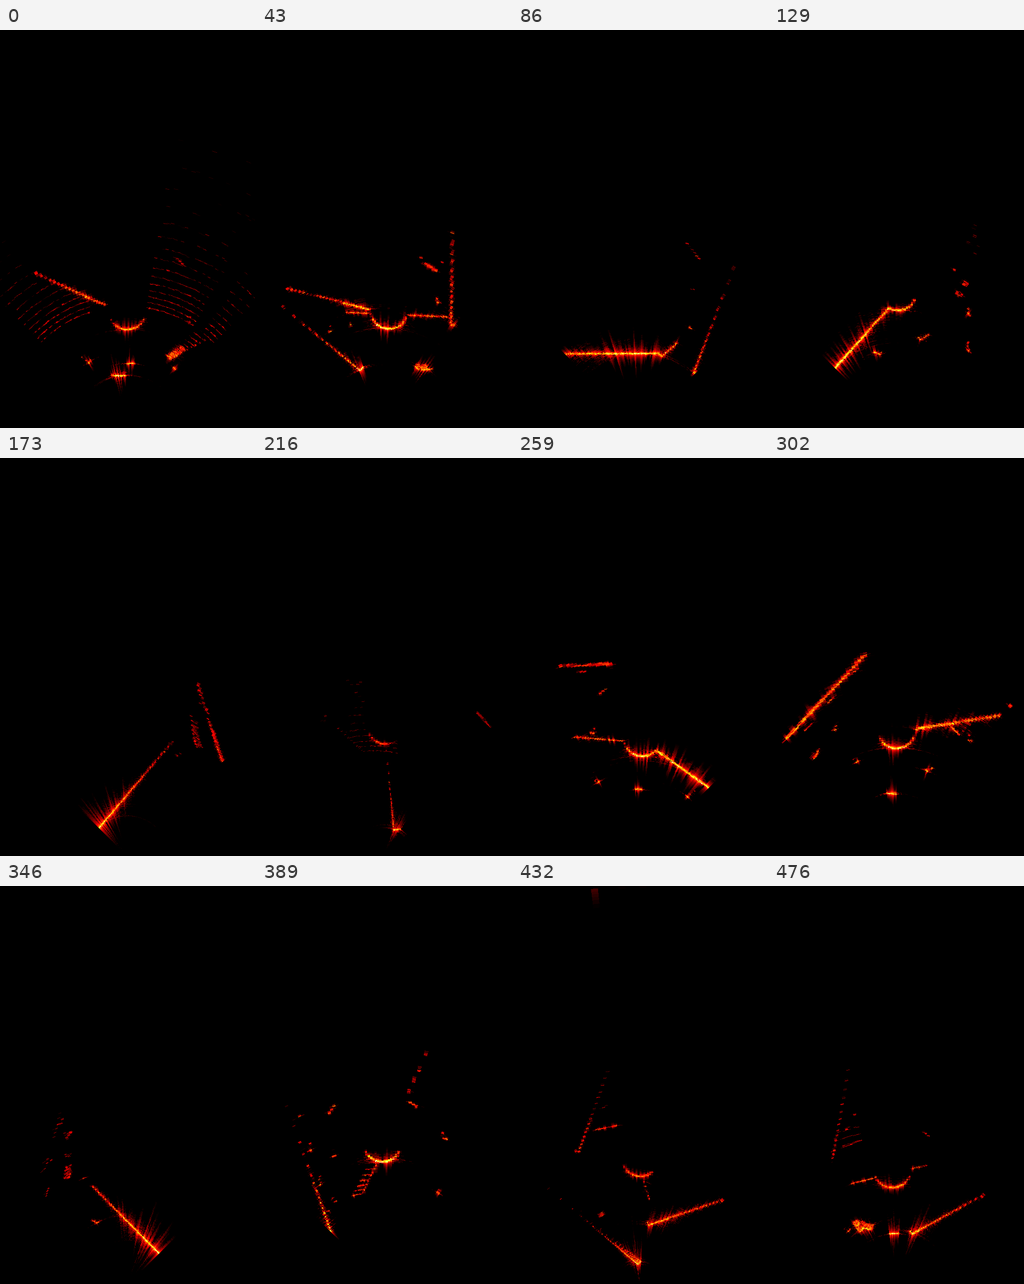
\includegraphics[width=\linewidth,height=0.73\textheight,keepaspectratio]{appendix_passA_recorded_sonar_contact_sheet.png}
			\end{center}
		\end{column}
	\end{columns}
\end{frame}

%------------------------------------------------

\begin{frame}
	\frametitle{From Simulated Geometry To NAS-GS Map}
	\framesubtitle{The learned map}

	\vspace{-1mm}
	{\footnotesize
	The two rows use the same top, side, and oblique projections. They differ because the DAVE row shows the full simulated target geometry, while the NAS-GS row shows Gaussian centres learned only from sonar-visible acoustic returns.
	}

	\vspace{1mm}
	\begin{center}
		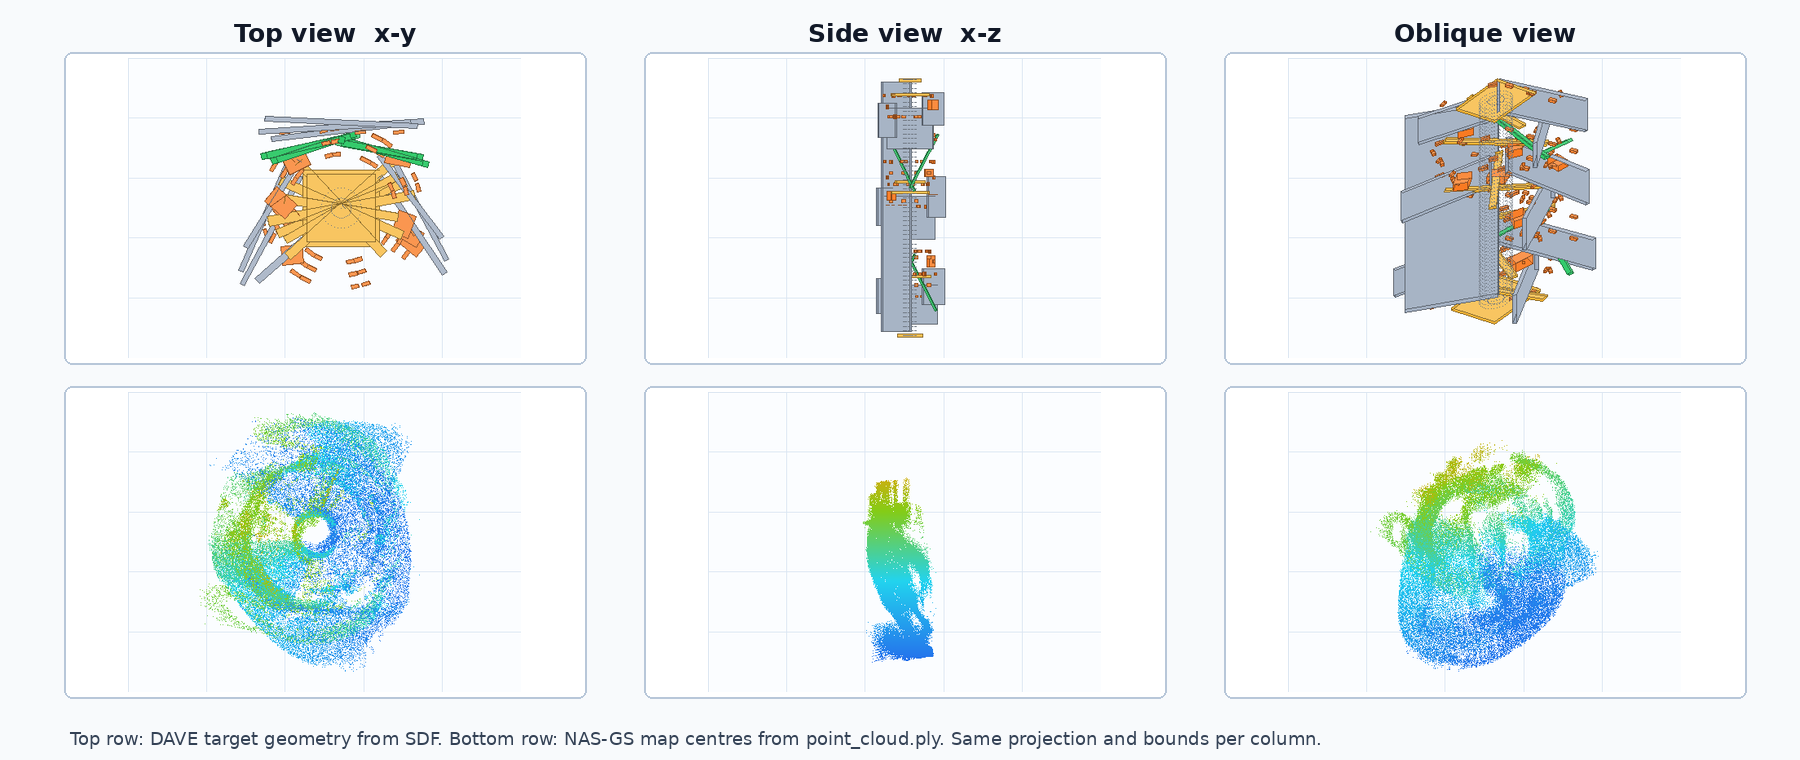
\includegraphics[width=0.99\textwidth,height=0.69\textheight,keepaspectratio]{passA_dave_vs_nasgs_sixpanel_slide.png}
	\end{center}
\end{frame}
\begin{frame}
	\frametitle{Experimental Design}
	\framesubtitle{Recorded data, map training, and replay policy}

	\begin{table}
		\scriptsize
		\renewcommand{\arraystretch}{1.15}
		\begin{tabular}{@{}p{0.14\textwidth}p{0.14\textwidth}p{0.15\textwidth}p{0.20\textwidth}p{0.25\textwidth}@{}}
			\toprule
			Case & Images & Sonar setting & NAS-GS map & Replay policy \\
			\midrule
			Pass A & 477 & \(90^\circ\), 20 m & Pass A 900k/i1000, PSNR 35.77 dB & Local single \\
			Pass A revisit & 431 & \(90^\circ\), 20 m & Pass A 900k/i1000, PSNR 35.77 dB & Local single; route-progress check \\
			Pass B revisit & 496 & \(90^\circ\), 20 m & Pass A 900k/i1000, PSNR 35.77 dB & Route-progress sequence \\
			Offshore & 1139 & \(120^\circ\), 12 m & Offshore 750k/i800, PSNR 33.68 dB & Local single \\
			\bottomrule
		\end{tabular}
	\end{table}

	\vspace{2mm}
	\textbf{Baseline setting}\\[-0.5mm]
	{\scriptsize IMU/DVL Pose3 replay with NAS-GS factors disabled. Noise is injected as DVL scale \(1.10\), body bias \((0.030,-0.025,0.0)\) m/s, yaw drift \(8.0{\times}10^{-4}\) rad/s, and 2.5 s DVL dropout every 35 s after 45 s.}
\end{frame}

%------------------------------------------------

\begin{frame}
	\frametitle{Pass A Policy Selection}
	\framesubtitle{The BP-rendered library with runtime no-BP scoring was selected}

	\begin{center}
		\setlength{\fboxsep}{4pt}
		\fcolorbox{ICLBlue}{ICLCream}{%
			\begin{minipage}{0.90\textwidth}
				\footnotesize
				\textbf{BP means beam-pattern rendering.}
				It applies the sonar's angular transmit/receive sensitivity as an intensity weighting, attenuating returns away from the central beam.
				\textbf{no-BP} omits this directional modulation.
			\end{minipage}}
	\end{center}
	\vspace{-0.5mm}

	\begin{center}
		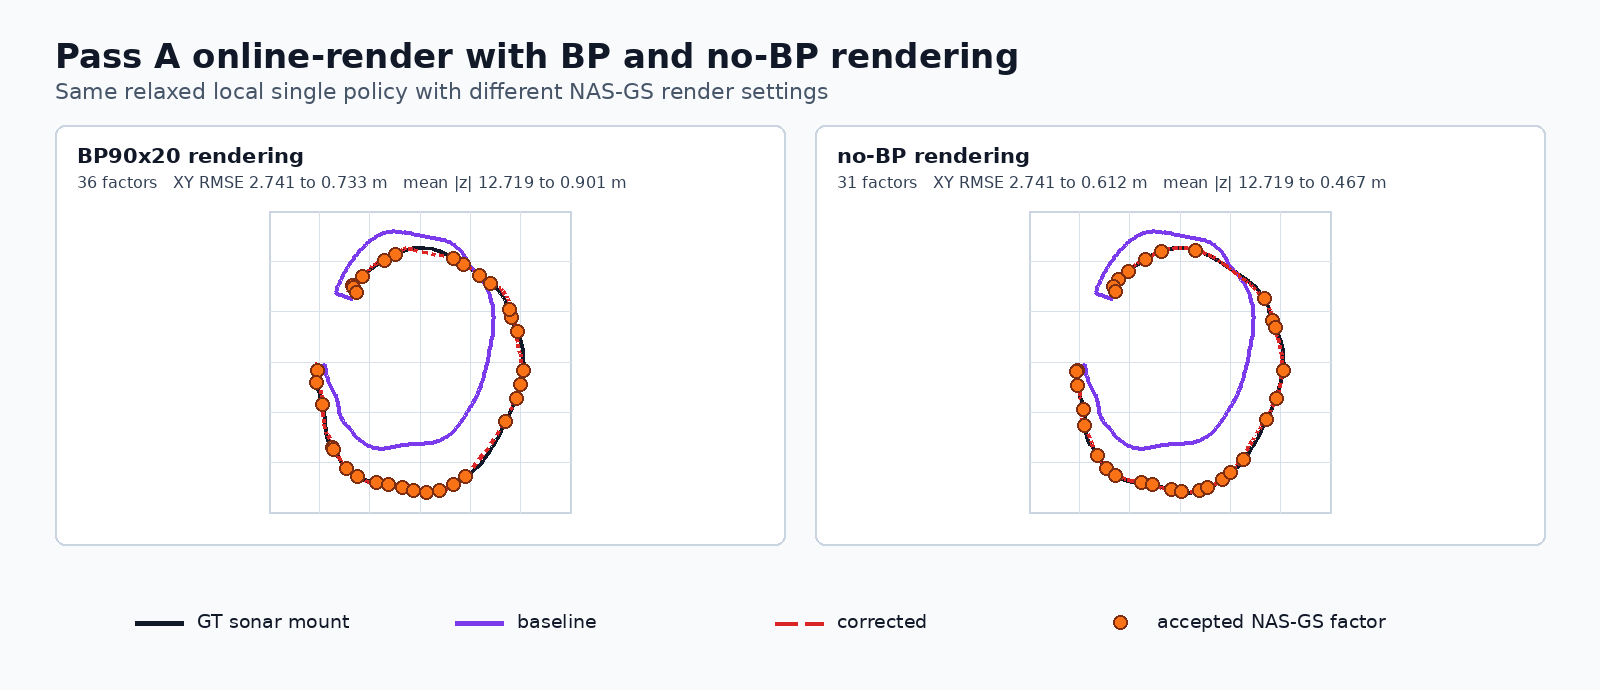
\includegraphics[width=0.82\textwidth,trim=0 0 0 112,clip]{passA_bp_vs_nobp_online_render_comparison.png}
	\end{center}
\end{frame}

%------------------------------------------------

\begin{frame}
	\frametitle{Pass A Sonar Evidence}
	\framesubtitle{One recorded frame and the corresponding BP/no-BP rendered libraries}

	\begin{columns}[T]
		\begin{column}{0.31\textwidth}
			\storycard{ICLCream}{ICLBlue}{Recorded Pass A}
			{Live sonar frame from the DAVE route.}
			\vspace{1mm}
			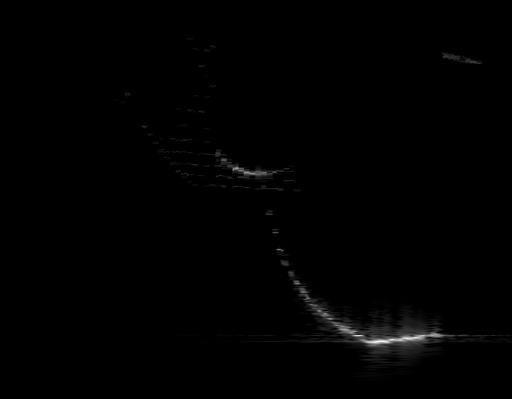
\includegraphics[width=\textwidth]{passA_evidence_live_frame216.png}
		\end{column}
		\begin{column}{0.31\textwidth}
			\storycard{ICLCream}{ICLBlue}{Rendered BP library}
			{Reference image from the trained NAS-GS map.}
			\vspace{1mm}
			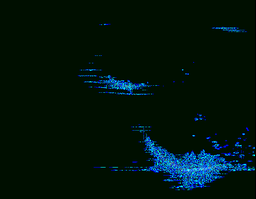
\includegraphics[width=\textwidth]{passA_evidence_rendered_bp_frame216.png}
		\end{column}
		\begin{column}{0.31\textwidth}
			\storycard{ICLCream}{ICLBlue}{Rendered no-BP library}
			{Alternative rendered appearance for policy testing.}
			\vspace{1mm}
			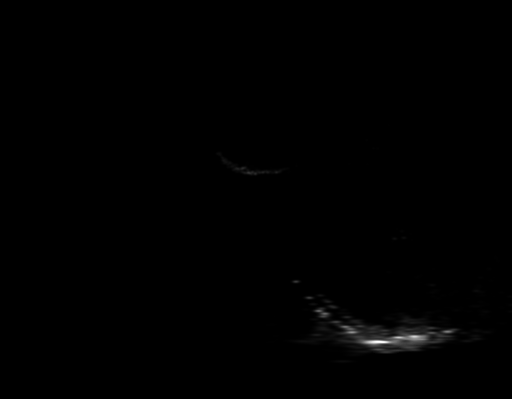
\includegraphics[width=\textwidth]{passA_evidence_rendered_nobp_frame216.png}
		\end{column}
	\end{columns}
\end{frame}

%------------------------------------------------

\begin{frame}
	\frametitle{Pass A Result}

	\begin{center}
		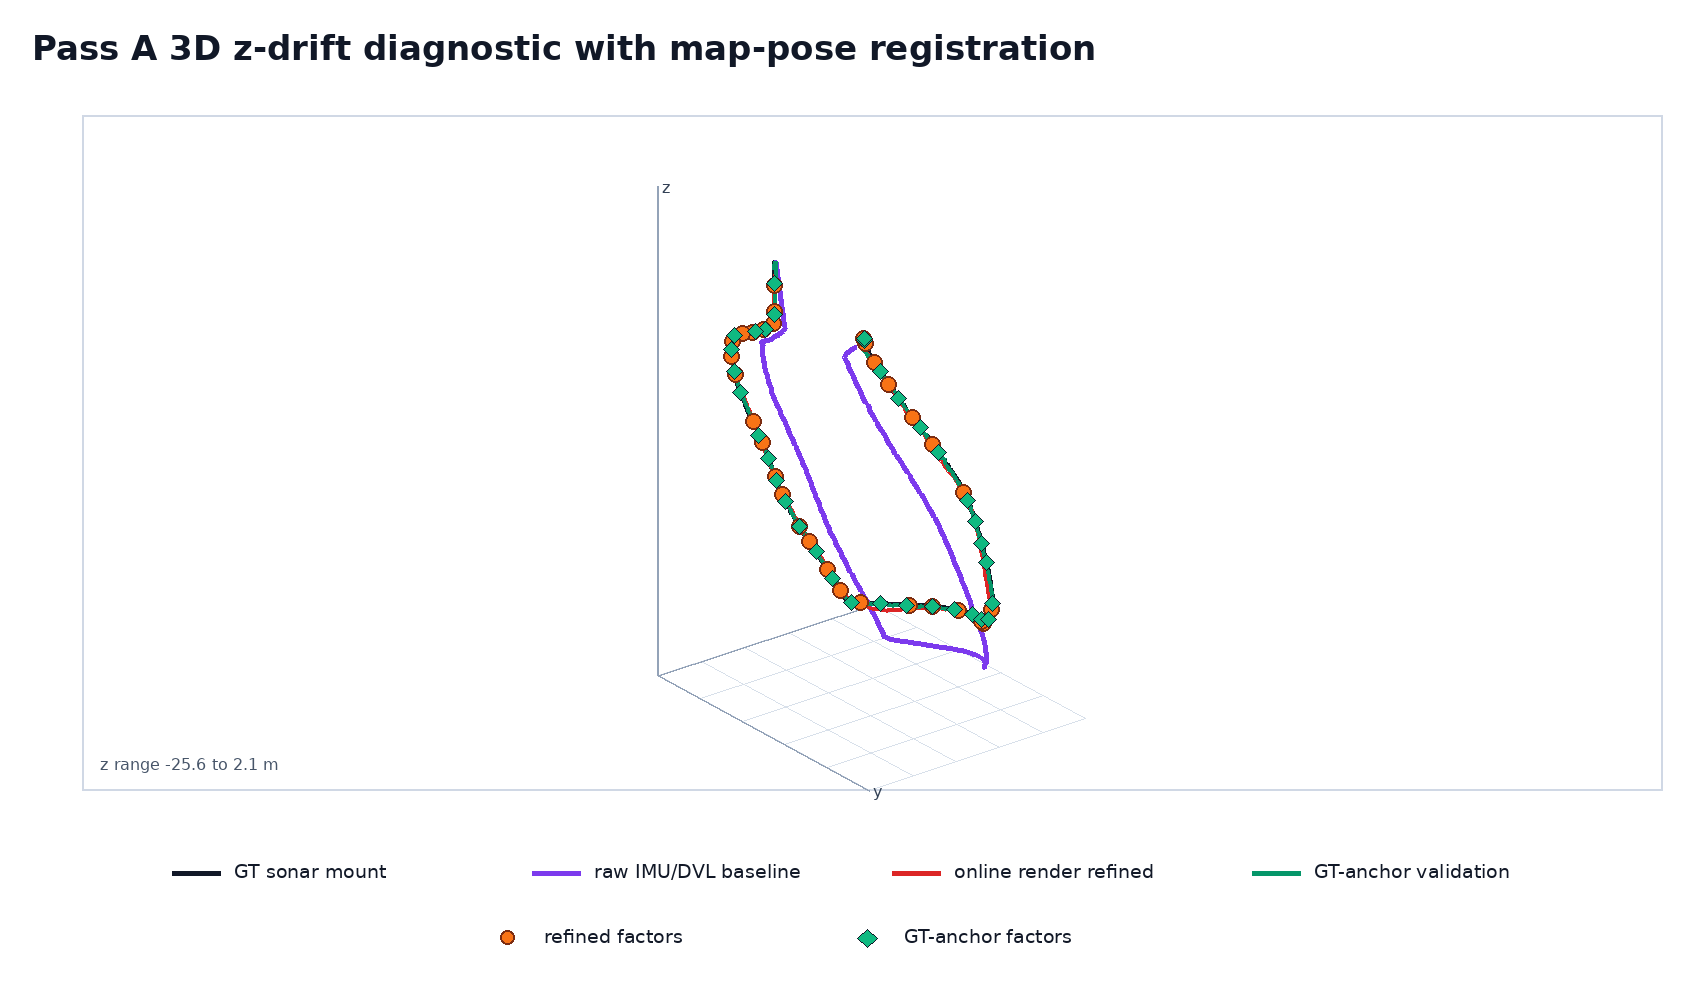
\includegraphics[height=0.75\textheight,keepaspectratio]{passA_current_online_render_3d_slidecrop.png}
	\end{center}
	\vspace{-2.5mm}
	\begin{center}
		{\scriptsize\textbf{Metrics:} 30 factors. XY RMSE \(2.741\to0.570\) m; XYZ RMSE \(15.078\to0.937\) m; mean \(|z|\) \(12.719\to0.569\) m.\\
		\textbf{Final error:} XY \(0.305\) m; \(|z|=0.069\) m.}
	\end{center}
\end{frame}

%------------------------------------------------

\begin{frame}
	\frametitle{Offshore Dataset: Real Sonar Validation}
	\framesubtitle{Wind-turbine inspection sequence}

	\begin{columns}[T]
		\begin{column}{0.63\textwidth}
			\begin{itemize}\small
				\setlength{\itemsep}{0.8mm}
				\item Real sequence recorded around an offshore wind-turbine foundation with a Tritech Gemini 1200ik imaging sonar.
				\item More than 20 minutes and \textbf{1,139 frames} from the surface towards the seabed, using a $120^\circ$ field of view and 12 m range.
				\item Sidelobe, speckle, multipath, and strong vertical motion make this a demanding real-acoustic transfer case.
			\end{itemize}
		\end{column}
		\begin{column}{0.31\textwidth}
			\storycard{ICLCream}{ICLBlue}{Reference and validation role}
			{Aqua-SLAM 6-DoF poses supervise NAS-GS and provide the replay reference. This is not independent survey ground truth.}
		\end{column}
	\end{columns}

	\vspace{1.5mm}
	\begin{columns}[T]
		\begin{column}{0.32\textwidth}
			\centering
			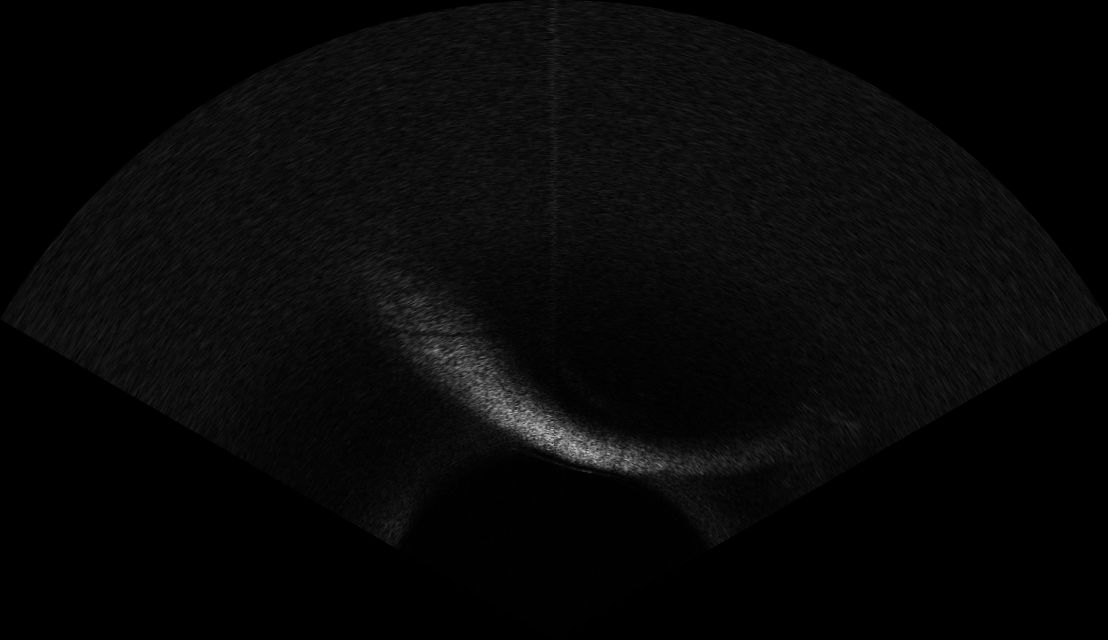
\includegraphics[width=\linewidth]{offshore_real_frame216.png}\\[-0.5mm]
			{\scriptsize Frame 216: strong curved return}
		\end{column}
		\begin{column}{0.32\textwidth}
			\centering
			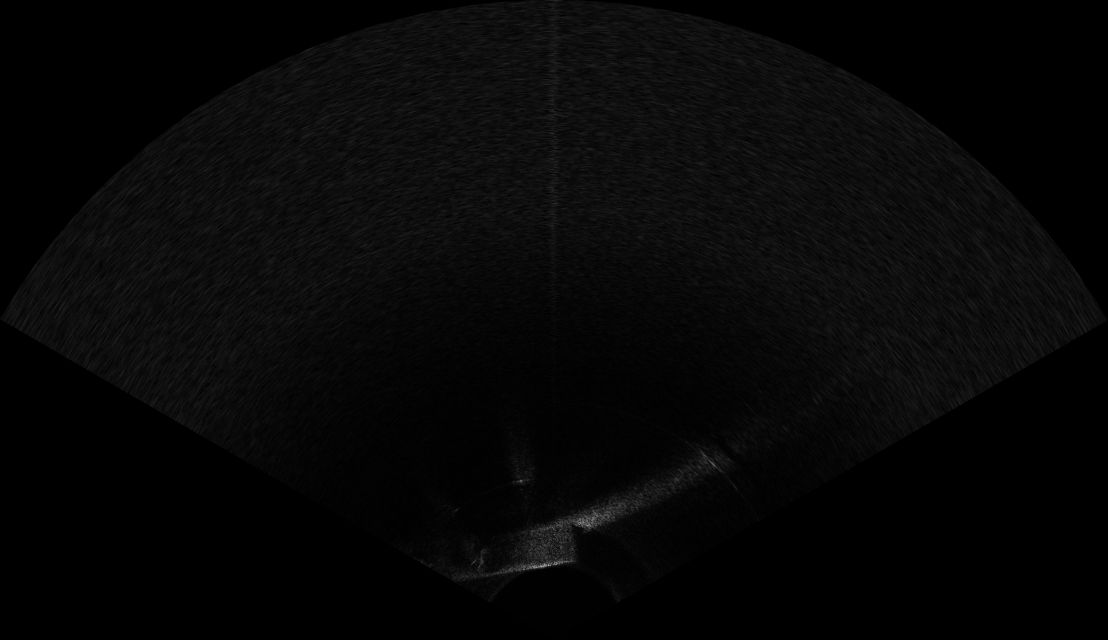
\includegraphics[width=\linewidth]{offshore_real_frame517.png}\\[-0.5mm]
			{\scriptsize Frame 517: partial return}
		\end{column}
		\begin{column}{0.32\textwidth}
			\centering
			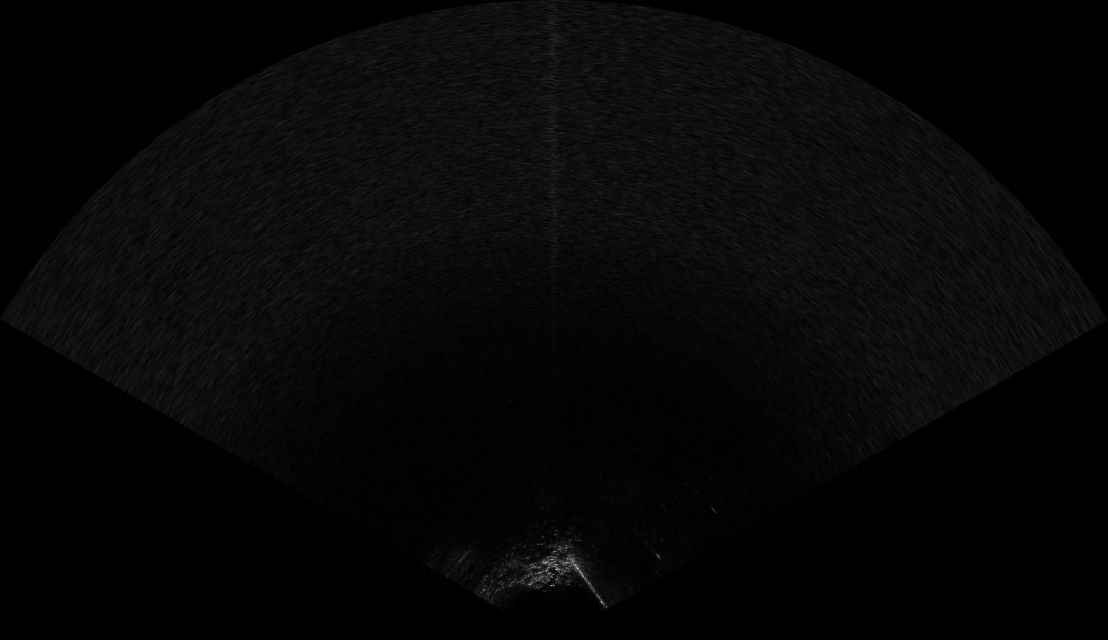
\includegraphics[width=\linewidth]{offshore_real_frame864.png}\\[-0.5mm]
			{\scriptsize Frame 864: sparse near-range return}
		\end{column}
	\end{columns}
\end{frame}

%------------------------------------------------

\begin{frame}
	\frametitle{BP versus no-BP on Offshore Data}
	\framesubtitle{The better rendering mode depends on the recorded sonar appearance}

	\begin{center}
		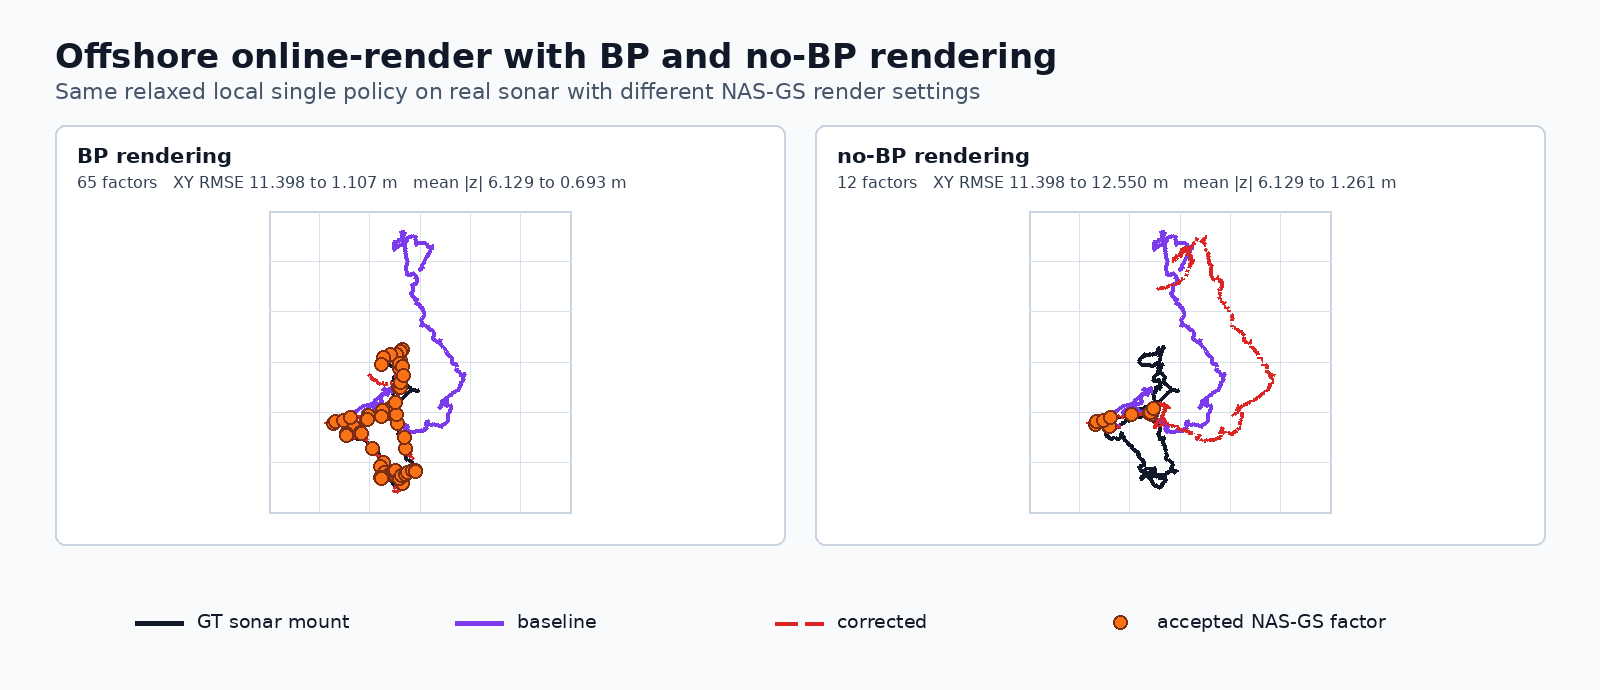
\includegraphics[width=0.82\textwidth]{offshore_bp_vs_nobp_online_render_comparison.png}
	\end{center}

	\vspace{-2mm}
	\scriptsize
	Offshore data contains stronger real-image artefacts, so BP and no-BP rendering are less interchangeable than in the DAVE Pass A replay.
\end{frame}

%------------------------------------------------

\begin{frame}
	\frametitle{Offshore Sonar Evidence}
	\framesubtitle{The real replay has stronger appearance mismatch than the DAVE route}

	\begin{columns}[T]
		\begin{column}{0.35\textwidth}
			\storycard{ICLCream}{ICLBlue}{Recorded offshore}
			{Live sonar from the replay.}
			\vspace{1mm}
			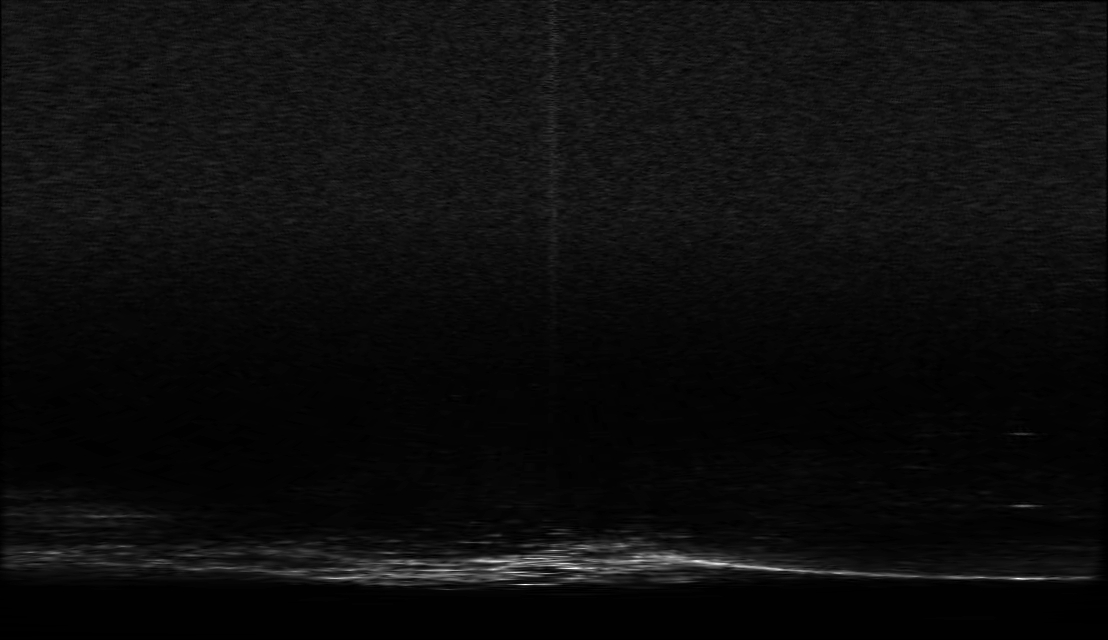
\includegraphics[width=\textwidth]{offshore_evidence_live_frame864.png}
		\end{column}
		\begin{column}{0.31\textwidth}
			\storycard{ICLCream}{ICLBlue}{Rendered BP library}
			{NAS-GS render with the offshore BP library.}
			\vspace{1mm}
			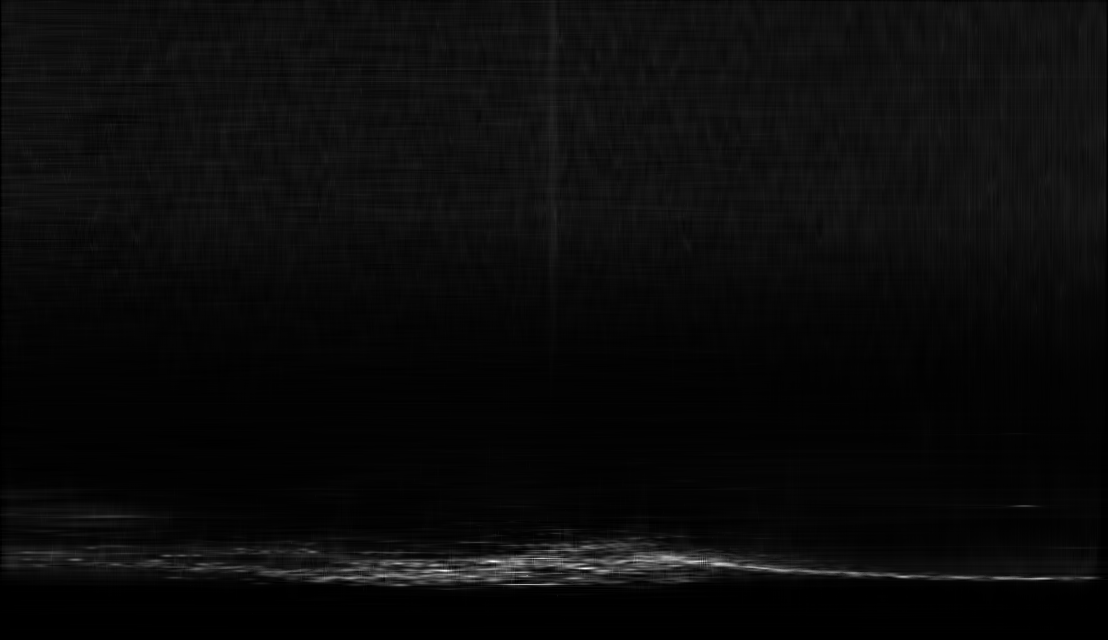
\includegraphics[width=\textwidth]{offshore_evidence_rendered_bp_frame864.png}
		\end{column}
		\begin{column}{0.31\textwidth}
			\storycard{ICLCream}{ICLBlue}{Rendered no-BP library}
			{No-BP render used for appearance comparison.}
			\vspace{1mm}
			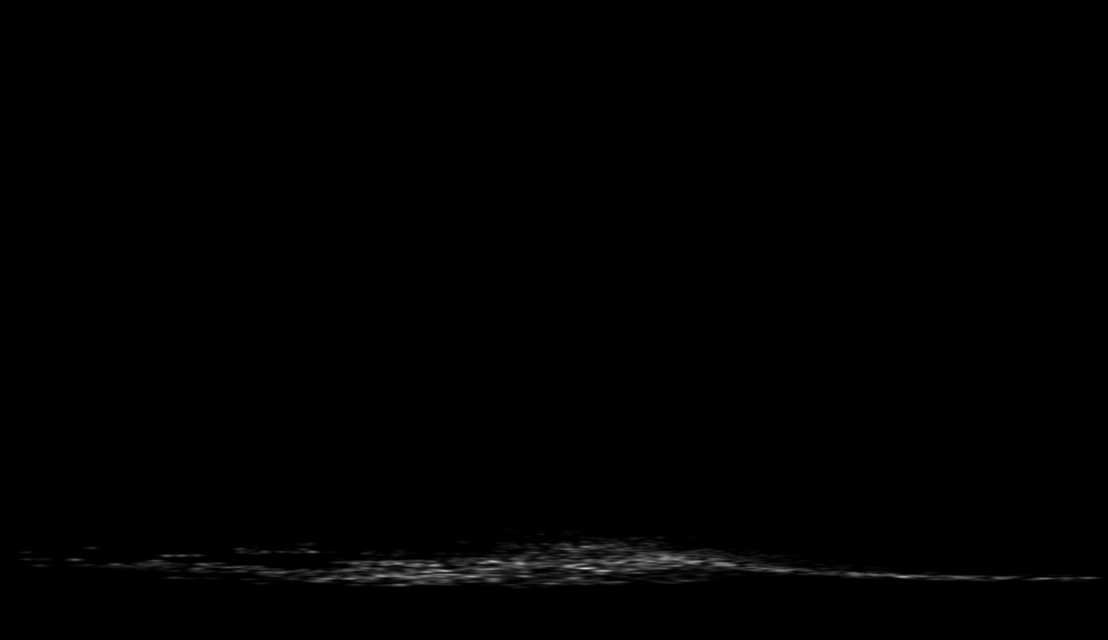
\includegraphics[width=\textwidth]{offshore_evidence_rendered_nobp_frame864.png}
		\end{column}
	\end{columns}
\end{frame}

%------------------------------------------------

\begin{frame}
	\frametitle{Offshore Validation}
	\framesubtitle{The method transfers, but the real-scene case exposes z and appearance limits}

	\begin{center}
		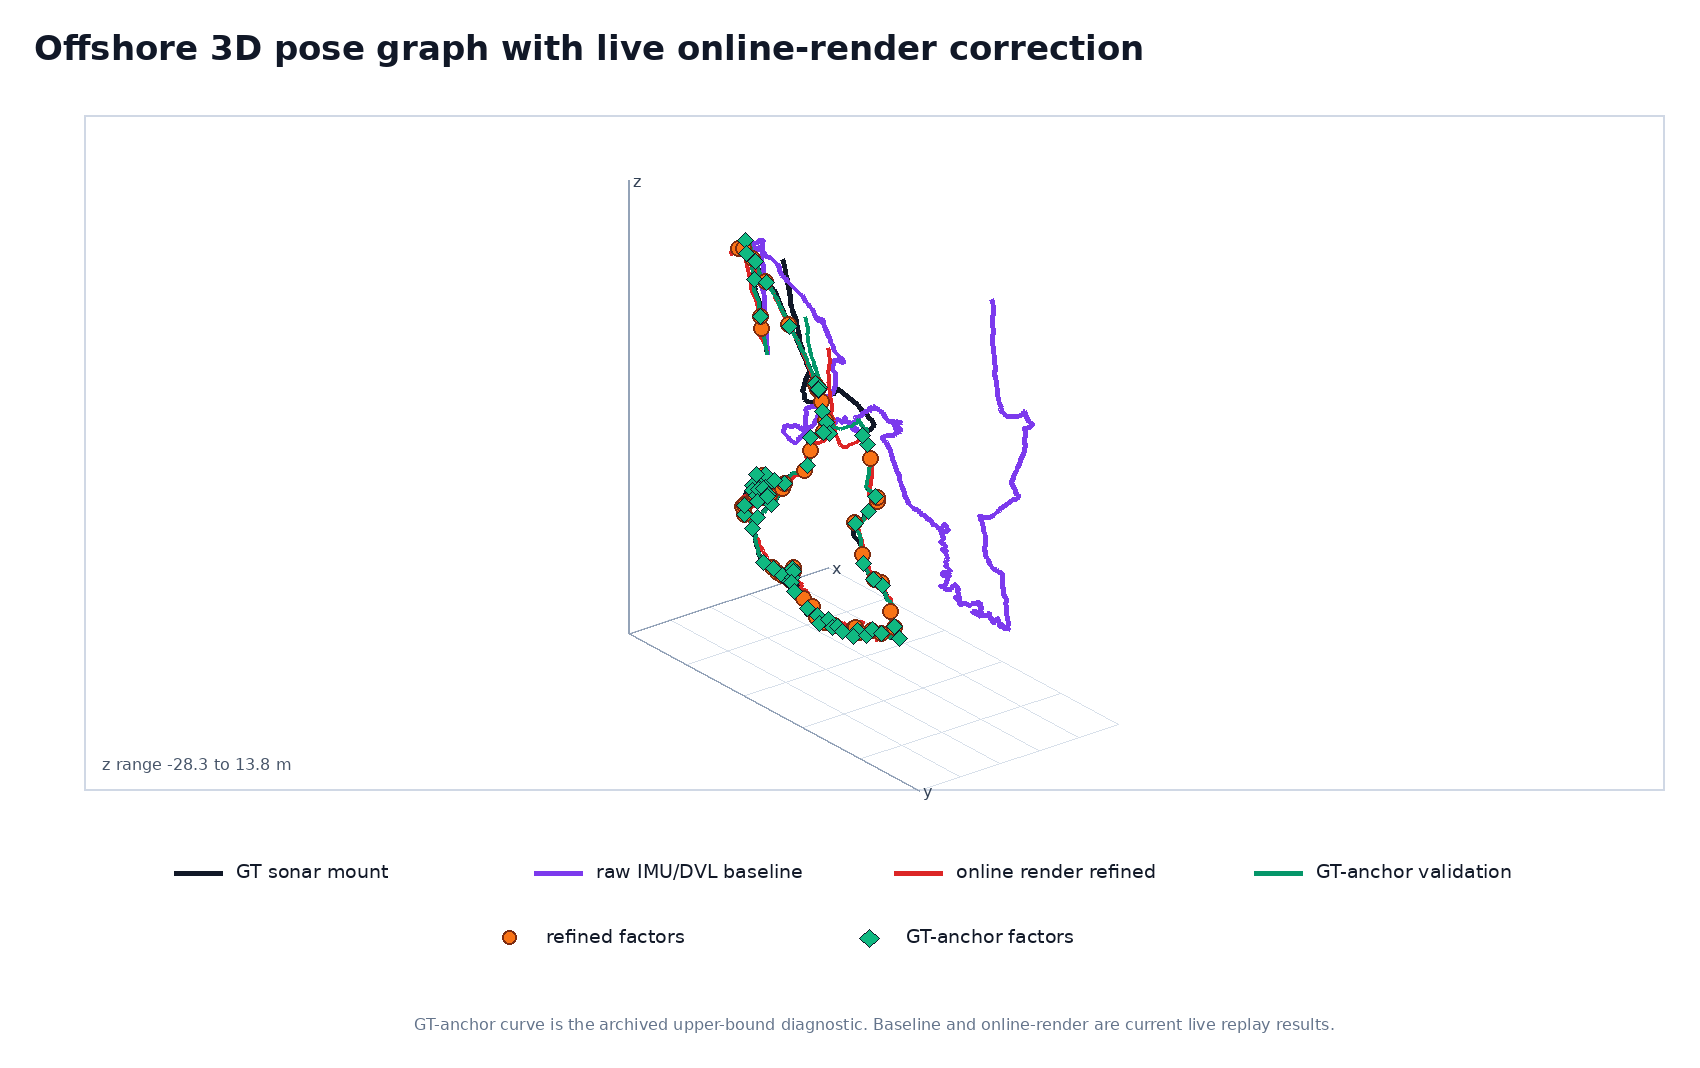
\includegraphics[height=0.7\textheight,keepaspectratio]{offshore_current_online_render_3d_slidecrop.png}
	\end{center}
	\vspace{-2.5mm}
	\begin{center}
		{\scriptsize\textbf{Metrics:} 50 factors. XY RMSE \(11.043\to1.407\) m; XYZ RMSE \(12.795\to2.126\) m; mean \(|z|\) \(6.074\to1.027\) m.\\
		\textbf{Final error:} XY \(9.843\) m; \(|z|=3.601\) m.}
	\end{center}
\end{frame}

%------------------------------------------------

\begin{frame}
	\frametitle{Revisit Baselines}
	\framesubtitle{Pass A revisit is same-route; Pass B is harder because the route direction changes}

	\begin{center}
		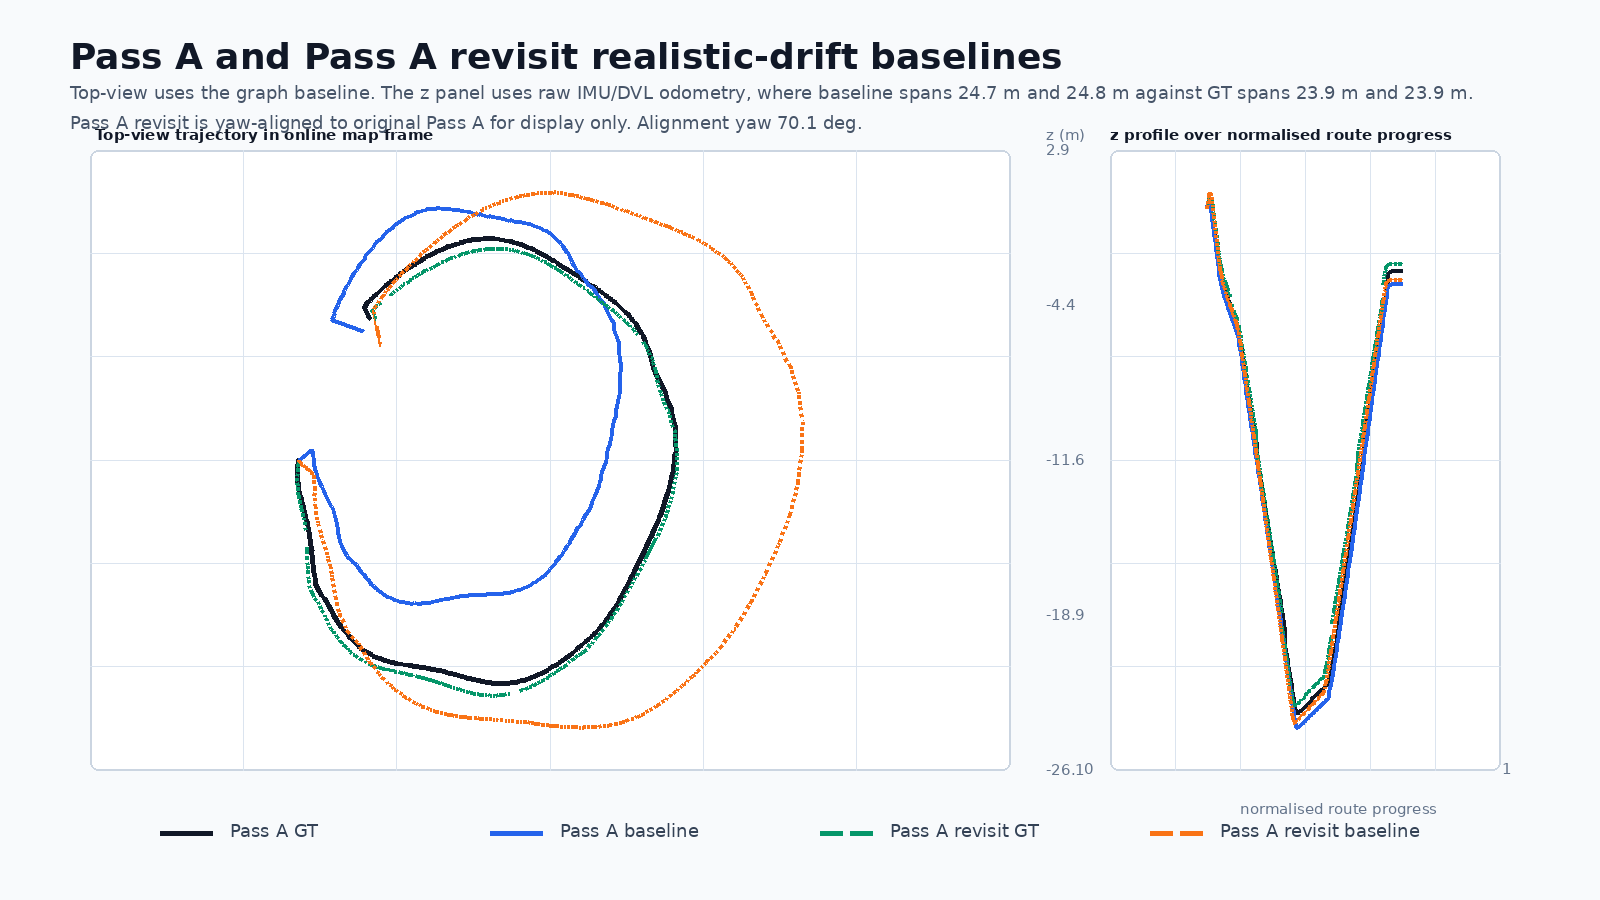
\includegraphics[width=0.9\textwidth]{passA_passA_revisit_baseline_overlay.png}
	\end{center}
\end{frame}

%------------------------------------------------

\begin{frame}
	\frametitle{Revisit Result}
	\framesubtitle{The revisit policy improves the hard case conservatively}

	\begin{center}
		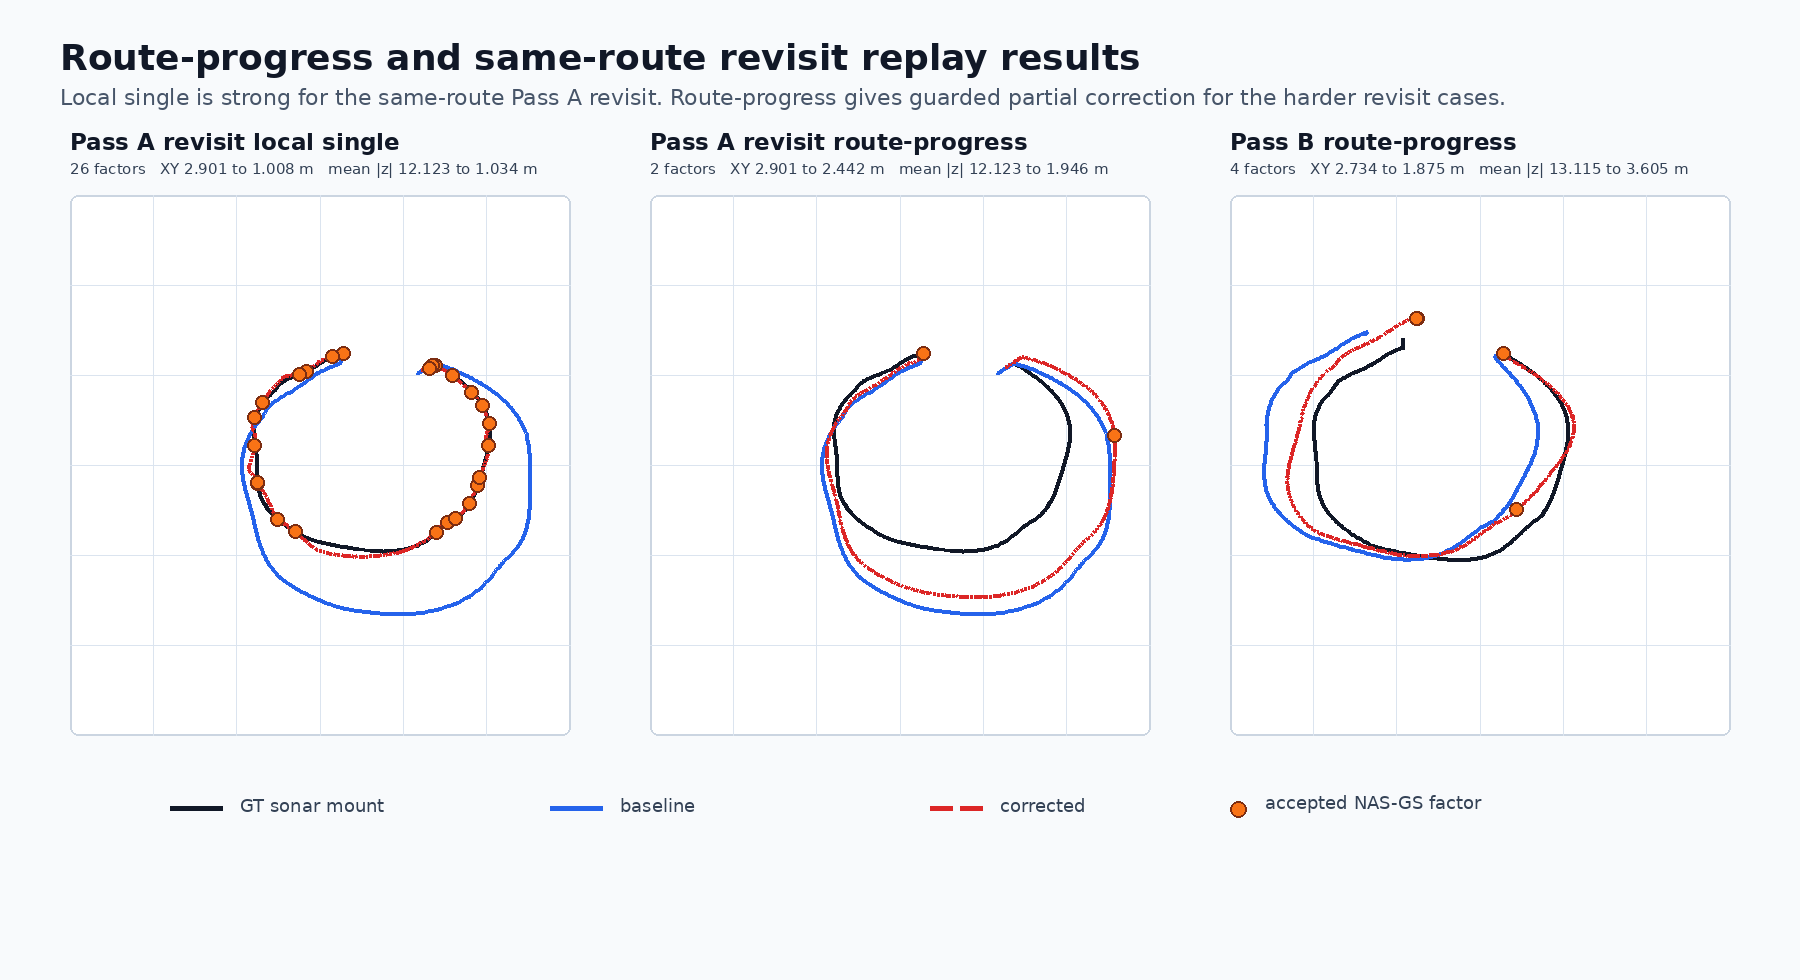
\includegraphics[width=0.9\textwidth]{route_progress_revisit_results.png}
	\end{center}
\end{frame}

%------------------------------------------------


\begin{frame}
	\frametitle{Limitations and Future Work}
	\framesubtitle{The next steps follow directly from the observed failure modes}

	\begin{columns}[T]
		\begin{column}{0.48\textwidth}
			\storycard{ICLCream}{ICLBlue}{Current limitations}
			{The remaining weaknesses define the operating boundary.}
			\begin{itemize}
				\item The current system is evaluated through live replay and does not yet estimate a complete 6-DoF correction.
				\item The NAS-GS Gaussian map is fixed during localisation and cannot adapt to map or appearance changes.
				\item Route-progress registration provides only limited improvement under the most difficult revisit conditions.
			\end{itemize}
		\end{column}
		\begin{column}{0.48\textwidth}
			\storycard{ICLBlue!6}{ICLBlue}{Key future work}
			{Each direction targets one demonstrated limitation.}
			\begin{itemize}
				\item Move from live replay to onboard timing, calibration, and safety trials with 6-DoF estimation.
				\item Retrain NAS-GS on corrected trajectories and validate against an independent reference.
				\item Use sequence-level optimisation for robust large-drift recovery.
				\item Add differentiable sonar-intensity error for continuous pose refinement beyond discrete gates.
			\end{itemize}
		\end{column}
	\end{columns}
\end{frame}

%------------------------------------------------

\begin{frame}
	\frametitle{Main Contributions}

	\vspace{4mm}
	\begin{itemize}
		\item \textbf{Integrated simulation framework}\quad DAVE data collection, NAS-GS training, and a live ROS Pose3 SLAM system.
		\item \textbf{Real-data-validated registration policies}\quad Controlled IMU/DVL baselines and gated online-render factors for pose-graph correction.
		\item \textbf{Foundation for sonar-based 3DGS SLAM}\quad A working connection from renderable sonar maps to incremental iSAM2 constraints.
	\end{itemize}
	\end{frame}

%------------------------------------------------

{
\setbeamercolor{background canvas}{bg=ICLBlue}
\begin{frame}[plain]
	\vspace{14mm}
	\begin{center}
		
\includegraphics[width=45mm]{ICL_Logo_White.pdf}

		\vspace{12mm}
		{\color{white}\Huge Thank you}

		\vspace{4mm}
		{\color{white}\Large Questions?}
	\end{center}
\end{frame}
}

\end{document}
